\documentclass[a4paper]{article}

\def\npart {UB PHC 607/608/609}
\def\nterm {Clinical pharmacokinetics and pharmacodynamics}
\def\nyear {2026}
\def\nlecturer {Guohua An's Buffalo notebooks, rewritten as an original study text}
\def\ncourse {Clinical PK/PD as Dose Individualization}
\def\ncoursehead {Clinical PK/PD}
\def\nauthor {NanFangHong}

\RequirePackage{etex}
\makeatletter
\ifx \npart \undefined
  \def\npart{PK/PD Notes}
\fi
\ifx \nterm \undefined
  \def\nterm{Reading notes}
\fi
\ifx \nyear \undefined
  \def\nyear{\the\year}
\fi
\ifx \nlecturer \undefined
  \def\nlecturer{the source literature}
\fi
\ifx \nauthor \undefined
  \def\nauthor{NanFangHong}
\fi
\ifx \ncourse \undefined
  \def\ncourse{Pharmacology Reading Note}
\fi
\ifx \ncoursehead \undefined
  \def\ncoursehead{\ncourse}
\fi

\author{Based on \nlecturer \\\small Notes taken by \nauthor}
\date{\nterm\ \nyear}
\title{\npart\ --- \ncourse}

\usepackage{amsfonts}
\usepackage{amsmath}
\usepackage{amssymb}
\usepackage{amsthm}
\usepackage{booktabs}
\usepackage{caption}
\usepackage{enumitem}
\usepackage{fancyhdr}
\usepackage{fontspec}
\usepackage{graphicx}
\usepackage{iftex}
\usepackage{mathtools}
\usepackage{microtype}
\usepackage{siunitx}
\usepackage{tabularx}
\usepackage{tikz}
\usepackage{xcolor}
\usepackage{xurl}
\usepackage{xeCJK}

\IfFontExistsTF{Latin Modern Roman}{
  \setmainfont[Ligatures=NoCommon]{Latin Modern Roman}
}{}

\IfFontExistsTF{Noto Serif CJK SC}{
  \setCJKmainfont{Noto Serif CJK SC}
}{
  \IfFontExistsTF{Songti SC}{
    \setCJKmainfont{Songti SC}
  }{
    \IfFontExistsTF{PingFang SC}{
      \setCJKmainfont{PingFang SC}
    }{}
  }
}

\usepackage[hidelinks,unicode,breaklinks=true]{hyperref}
\hypersetup{
  pdfauthor={\nauthor},
  pdfsubject={\npart\ - \ncourse},
  pdftitle={\npart\ - \ncourse},
  pdfkeywords={PK PD pharmacology reading notes \ncourse}
}

\pagestyle{fancyplain}
\lhead{\emph{\nouppercase{\leftmark}}}
\rhead{
  \ifnum\thepage=1
  \else
    \npart\ \ncoursehead
  \fi}

\theoremstyle{definition}
\newtheorem*{aim}{Aim}
\newtheorem*{assumption}{Assumption}
\newtheorem*{defi}{Definition}
\newtheorem*{eg}{Example}
\newtheorem*{notation}{Notation}
\newtheorem*{question}{Question}
\newtheorem*{remark}{Remark}
\newtheorem*{warning}{Warning}

\theoremstyle{plain}
\newtheorem{nthm}{Theorem}[section]
\newtheorem{nprop}[nthm]{Proposition}

\renewcommand{\labelitemi}{--}
\renewcommand{\labelitemii}{$\circ$}
\renewcommand{\labelenumi}{(\roman{*})}

\let\stdsection\section
\renewcommand\section{\newpage\stdsection}

\newcommand{\dd}{\mathop{}\!\mathrm{d}}
\newcommand{\Emax}{E_{\max}}
\newcommand{\pksym}[1]{\ifmmode\text{\textit{#1}}\else\textit{#1}\fi}
\newcommand{\pklab}[1]{\mathrm{#1}}
\newcommand{\ECfifty}{\pksym{EC}_{50}}
\newcommand{\term}[1]{\emph{#1}}
\makeatother

\usetikzlibrary{arrows.meta,fit,positioning}
\definecolor{pkblue}{RGB}{43,103,160}
\definecolor{pkred}{RGB}{176,69,69}
\definecolor{pkgreen}{RGB}{70,138,96}
\definecolor{pkamber}{RGB}{190,130,45}
\definecolor{pklight}{RGB}{240,246,252}
\definecolor{pklightred}{RGB}{252,242,240}
\definecolor{pklightgreen}{RGB}{241,249,244}
\definecolor{pklightamber}{RGB}{252,247,236}

\tikzset{
  pkbox/.style={draw=pkblue, thick, rounded corners=2pt, fill=pklight, align=center, inner sep=4pt},
  pkboxred/.style={draw=pkred, thick, rounded corners=2pt, fill=pklightred, align=center, inner sep=4pt},
  pkboxgreen/.style={draw=pkgreen, thick, rounded corners=2pt, fill=pklightgreen, align=center, inner sep=4pt},
  pkboxamber/.style={draw=pkamber, thick, rounded corners=2pt, fill=pklightamber, align=center, inner sep=4pt},
  pkcomp/.style={draw=pkblue, thick, circle, fill=pklight, align=center, minimum size=1.35cm, inner sep=2pt},
  pkorgan/.style={draw=pkblue, thick, rounded corners=2pt, fill=pklight, align=center, minimum width=1.75cm, minimum height=.58cm},
  pkarr/.style={-{Stealth[length=2.2mm]}, thick, draw=pkblue},
  pkarrred/.style={-{Stealth[length=2.2mm]}, thick, draw=pkred},
  pkarrgreen/.style={-{Stealth[length=2.2mm]}, thick, draw=pkgreen},
  pkdash/.style={-{Stealth[length=2.2mm]}, thick, dashed, draw=pkamber}
}

\newsavebox{\pkfigbox}
\newcommand{\pkfitfigure}[1]{%
  \sbox{\pkfigbox}{#1}%
  \ifdim\wd\pkfigbox>0.96\linewidth
    \resizebox{0.96\linewidth}{!}{\usebox{\pkfigbox}}%
  \else
    \usebox{\pkfigbox}%
  \fi
}

\newcommand{\figureDecisionLoop}{
\begin{center}
\pkfitfigure{%
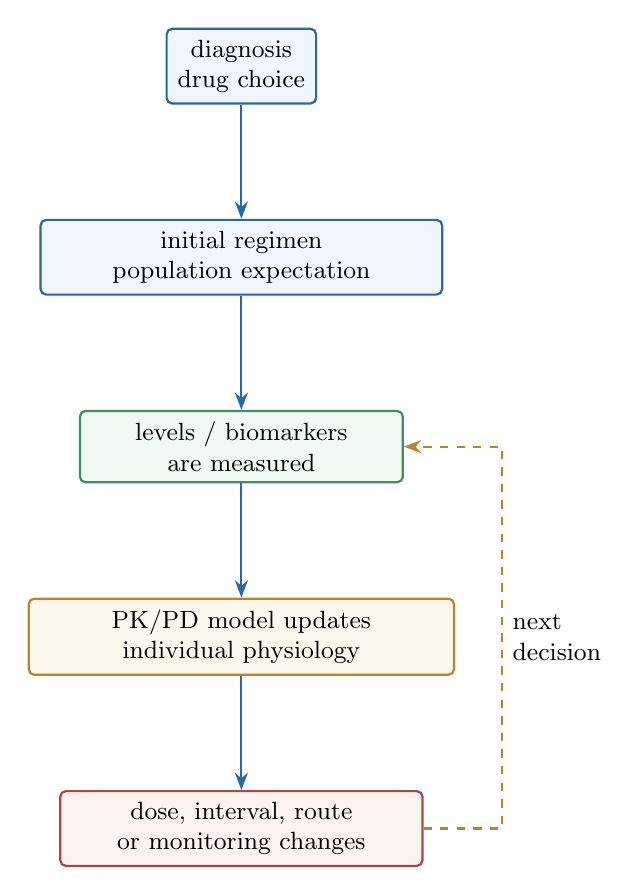
\begin{tikzpicture}[node distance=1.45cm and 1.55cm, font=\small]
  \node[pkbox] (diagnosis) {diagnosis\\drug choice};
  \node[pkbox, below=of diagnosis, minimum width=5.1cm] (start) {initial regimen\\population expectation};
  \node[pkboxgreen, below=of start, minimum width=4.1cm] (measure) {levels / biomarkers\\are measured};
  \node[pkboxamber, below=of measure, minimum width=5.4cm] (model) {PK/PD model updates\\individual physiology};
  \node[pkboxred, below=of model, minimum width=4.6cm] (change) {dose, interval, route\\or monitoring changes};
  \draw[pkarr] (diagnosis) -- (start);
  \draw[pkarr] (start) -- (measure);
  \draw[pkarr] (measure) -- (model);
  \draw[pkarr] (model) -- (change);
  \draw[pkdash] (change.east) -- ++(1.0,0) |- node[pos=.25,right,align=left] {next\\decision} (measure.east);
\end{tikzpicture}%
}
\captionof{figure}{A clinical PK/PD decision loop. This is an original redraw of the TDM workflow idea: diagnosis starts therapy, data update the model, and the next regimen is a decision under uncertainty.}
\end{center}
}

\newcommand{\figureCompartmentFamily}{
\begin{center}
\pkfitfigure{%
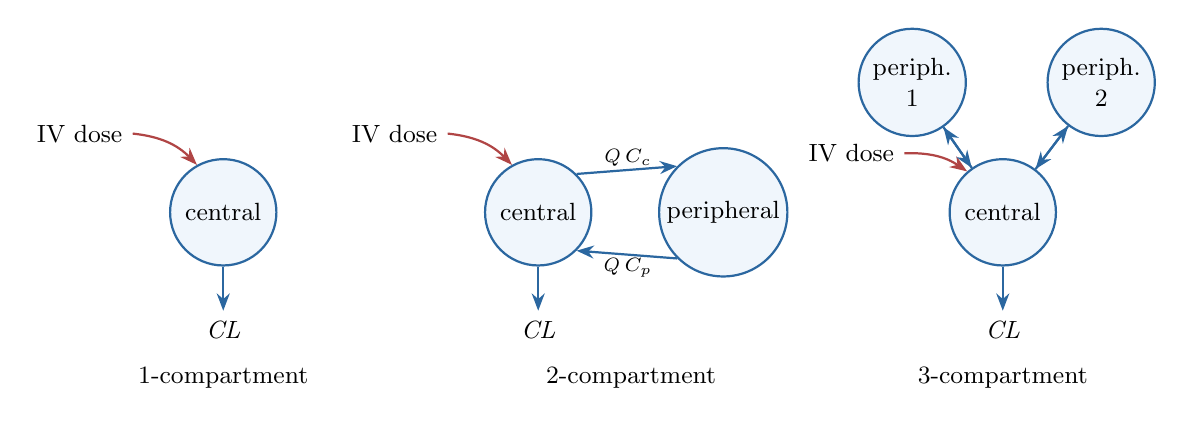
\begin{tikzpicture}[font=\small, x=1cm, y=1cm]
  \node[pkcomp] (c1) at (0,0) {central};
  \draw[pkarrred] (-1.15,1.0) node[left] {IV dose} to[bend left=20] (c1);
  \draw[pkarr] (c1) -- ++(0,-1.25) node[below] {\(\pkCL\)};
  \node at (0,-2.1) {1-compartment};

  \node[pkcomp] (c2) at (4.0,0) {central};
  \node[pkcomp] (p2) at (6.35,0) {peripheral};
  \draw[pkarrred] (2.85,1.0) node[left] {IV dose} to[bend left=20] (c2);
  \draw[pkarr] (c2) -- ++(0,-1.25) node[below] {\(\pkCL\)};
  \draw[pkarr] (c2.north east) -- node[above,font=\scriptsize,inner sep=1pt] {\(\pkQ\,C_c\)} (p2.north west);
  \draw[pkarr] (p2.south west) -- node[below,font=\scriptsize,inner sep=1pt] {\(\pkQ\,C_p\)} (c2.south east);
  \node at (5.18,-2.1) {2-compartment};

  \node[pkcomp] (c3) at (9.9,0) {central};
  \node[pkcomp] (p31) at (8.75,1.65) {periph.\\1};
  \node[pkcomp] (p32) at (11.15,1.65) {periph.\\2};
  \draw[pkarrred] (8.65,.75) node[left] {IV dose} to[bend left=18] (c3);
  \draw[pkarr] (c3) -- ++(0,-1.25) node[below] {\(\pkCL\)};
  \draw[pkarr] (c3) -- (p31);
  \draw[pkarr] (p31) -- (c3);
  \draw[pkarr] (c3) -- (p32);
  \draw[pkarr] (p32) -- (c3);
  \node at (9.9,-2.1) {3-compartment};
\end{tikzpicture}%
}
\captionof{figure}{Compartmental models as mass-balance diagrams. The central compartment receives input and elimination; peripheral compartments add distribution time scales without adding systemic clearance unless explicitly modeled. In the two-compartment panel, \(\pkQ\,C_c\) and \(\pkQ\,C_p\) are opposing distribution fluxes; the corresponding first-order rate constants are \(Q/V_c\) and \(Q/V_p\), not generally equal.}
\end{center}
}

\newcommand{\figureAbsorptionBarriers}{
\begin{center}
\pkfitfigure{%
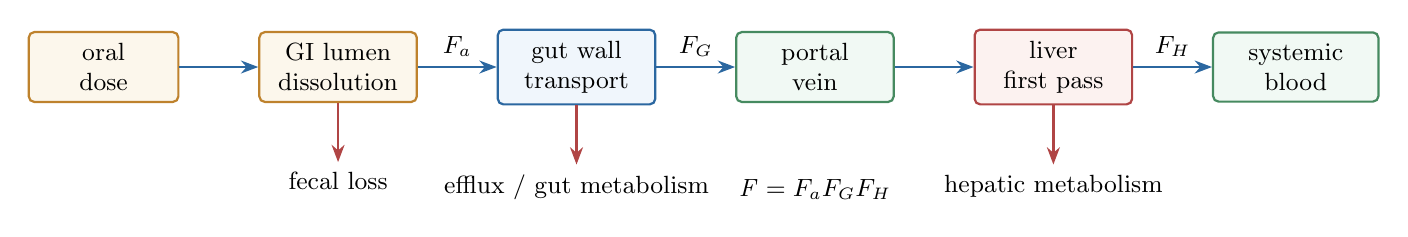
\begin{tikzpicture}[font=\small, node distance=.7cm and 1.0cm]
  \node[pkboxamber, minimum width=1.9cm] (dose) {oral\\dose};
  \node[pkboxamber, right=of dose, minimum width=2.0cm] (lumen) {GI lumen\\dissolution};
  \node[pkbox, right=of lumen, minimum width=2.0cm] (wall) {gut wall\\transport};
  \node[pkboxgreen, right=of wall, minimum width=2.0cm] (portal) {portal\\vein};
  \node[pkboxred, right=of portal, minimum width=2.0cm] (liver) {liver\\first pass};
  \node[pkboxgreen, right=of liver, minimum width=2.1cm] (sys) {systemic\\blood};
  \draw[pkarr] (dose) -- (lumen);
  \draw[pkarr] (lumen) -- node[above] {\(F_a\)} (wall);
  \draw[pkarr] (wall) -- node[above] {\(F_G\)} (portal);
  \draw[pkarr] (portal) -- (liver);
  \draw[pkarr] (liver) -- node[above] {\(F_H\)} (sys);
  \draw[pkarrred] (lumen.south) -- ++(0,-.75) node[below] {fecal loss};
  \draw[pkarrred] (wall.south) -- ++(0,-.75) node[below] {efflux / gut metabolism};
  \draw[pkarrred] (liver.south) -- ++(0,-.75) node[below] {hepatic metabolism};
  \node[below=.85cm of portal, align=center] {\(\pkF=F_aF_GF_H\)};
\end{tikzpicture}%
}
\captionof{figure}{Oral bioavailability as a sequence of barriers. The figure abstracts the gut--portal--liver structure from the source notebooks into the factorization \(F=F_aF_GF_H\).}
\end{center}
}

\newcommand{\figureAucTrapezoids}{
\begin{center}
\pkfitfigure{%
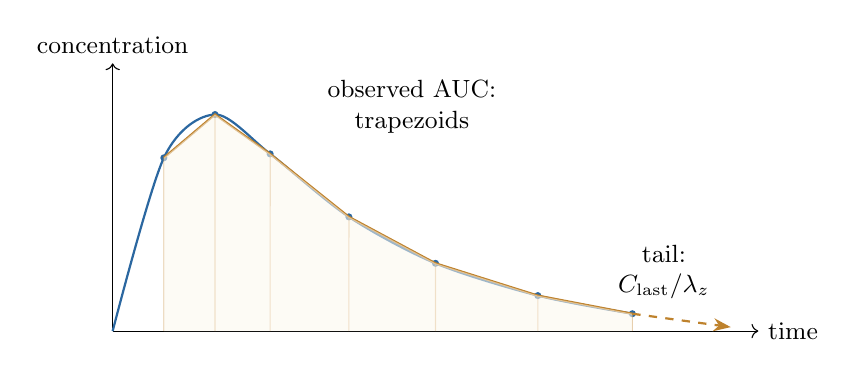
\begin{tikzpicture}[font=\small, x=1cm, y=1cm]
  \draw[->] (0,0) -- (8.2,0) node[right] {time};
  \draw[->] (0,0) -- (0,3.4) node[above] {concentration};
  \draw[thick, pkblue, smooth] plot coordinates {(0,0) (.65,2.2) (1.3,2.75) (2.0,2.25) (3.0,1.45) (4.1,.86) (5.4,.45) (6.6,.22)};
  \foreach \x/\y in {.65/2.2,1.3/2.75,2.0/2.25,3.0/1.45,4.1/.86,5.4/.45,6.6/.22} {
    \fill[pkblue] (\x,\y) circle (.045);
    \draw[draw=pkamber, fill=pklightamber, opacity=.45] (\x,0) -- (\x,\y) -- ++(.001,0) -- (\x,0);
  }
  \draw[pkamber, thick] (.65,2.2) -- (1.3,2.75) -- (2.0,2.25) -- (3.0,1.45) -- (4.1,.86) -- (5.4,.45) -- (6.6,.22);
  \fill[pklightamber, opacity=.55] (.65,0) -- (.65,2.2) -- (1.3,2.75) -- (2.0,2.25) -- (3.0,1.45) -- (4.1,.86) -- (5.4,.45) -- (6.6,.22) -- (6.6,0) -- cycle;
  \draw[pkdash] (6.6,.22) -- (7.85,.05);
  \node[align=center] at (3.8,2.85) {observed AUC:\\trapezoids};
  \node[align=center] at (7.0,.75) {tail:\\\(C_{\pklab{last}}/\lambda_z\)};
\end{tikzpicture}%
}
\captionof{figure}{NCA as curve geometry. The observed area is numerical geometry; the terminal tail is a model assumption about \(\lambda_z\).}
\end{center}
}

\newcommand{\figureMultipleDosing}{
\begin{center}
\pkfitfigure{%
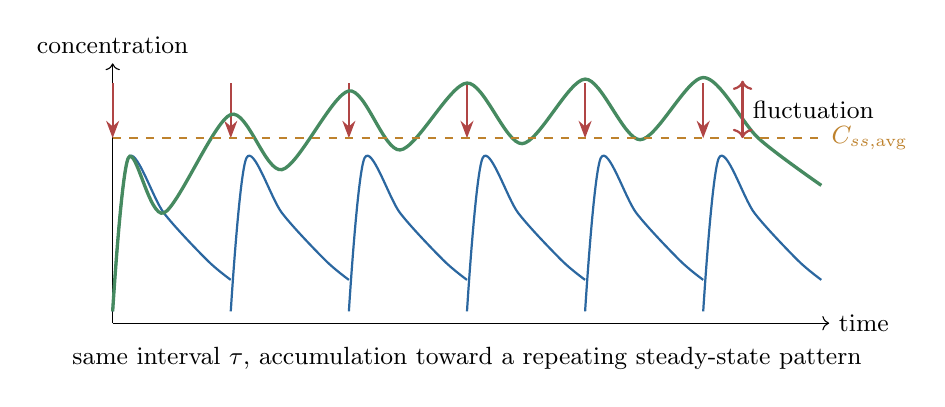
\begin{tikzpicture}[font=\small, x=1cm, y=1cm]
  \draw[->] (0,0) -- (9.1,0) node[right] {time};
  \draw[->] (0,0) -- (0,3.3) node[above] {concentration};
  \foreach \d in {0,1.5,3,4.5,6,7.5} {
    \draw[pkblue, thick, smooth] plot coordinates {(\d,0.15) (\d+.2,2.1) (\d+.65,1.4) (\d+1.2,.8) (\d+1.5,.55)};
    \draw[pkarrred] (\d,3.05) -- (\d,2.35);
  }
  \draw[pkgreen, very thick, smooth] plot coordinates {(0,.15) (.2,2.1) (.65,1.4) (1.5,2.65) (2.15,1.95) (3,2.95) (3.65,2.2) (4.5,3.05) (5.2,2.28) (6,3.1) (6.7,2.33) (7.5,3.12) (8.2,2.35) (9,1.75)};
  \draw[dashed, pkamber, thick] (0,2.35) -- (9,2.35) node[right] {\(\pkCavg\)};
  \draw[<->, thick, draw=pkred] (8.0,2.35) -- (8.0,3.08) node[midway,right] {fluctuation};
  \node at (4.5,-.45) {same interval \(\tau\), accumulation toward a repeating steady-state pattern};
\end{tikzpicture}%
}
\captionof{figure}{Multiple dosing by superposition. Repeated doses accumulate until the profile repeats; average exposure is clearance-controlled, while fluctuation is shaped by half-life and \(\tau\).}
\end{center}
}

\newcommand{\figureWellStirred}{
\begin{center}
\pkfitfigure{%
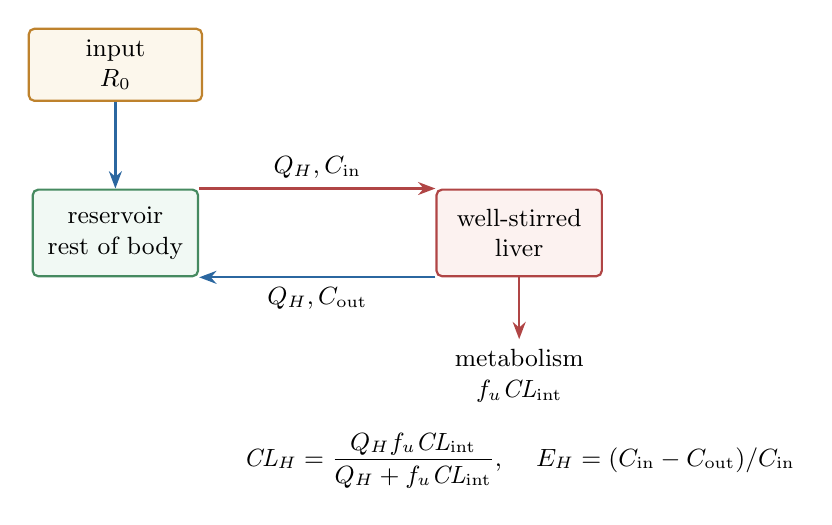
\begin{tikzpicture}[font=\small, node distance=1cm and 1.1cm]
  \node[pkboxgreen, minimum width=2.1cm, minimum height=1.1cm] (res) {reservoir\\rest of body};
  \node[pkboxred, right=3.0cm of res, minimum width=2.1cm, minimum height=1.1cm] (liv) {well-stirred\\liver};
  \draw[pkarrred] (res.north east) -- node[above] {\(Q_H, C_{\pklab{in}}\)} (liv.north west);
  \draw[pkarr] (liv.south west) -- node[below] {\(Q_H, C_{\pklab{out}}\)} (res.south east);
  \draw[pkarrred] (liv) -- ++(0,-1.35) node[below,align=center] {metabolism\\\(f_u\pkCL_{\pklab{int}}\)};
  \node[pkboxamber, above=1.1cm of res, minimum width=2.2cm] (input) {input\\\(R_0\)};
  \draw[pkarr] (input) -- (res);
  \node[below=1.85cm of liv, align=center] {\(\displaystyle \pkCL_H=\frac{Q_H f_u\pkCL_{\pklab{int}}}{Q_H+f_u\pkCL_{\pklab{int}}}\), \quad \(E_H=(C_{\pklab{in}}-C_{\pklab{out}})/C_{\pklab{in}}\)};
\end{tikzpicture}%
}
\captionof{figure}{Well-stirred hepatic clearance. This redraw keeps the source figure's core idea: blood flow brings drug into a mixed liver space where intrinsic capacity and binding determine extraction.}
\end{center}
}

\newcommand{\figureRenalHandling}{
\begin{center}
\pkfitfigure{%
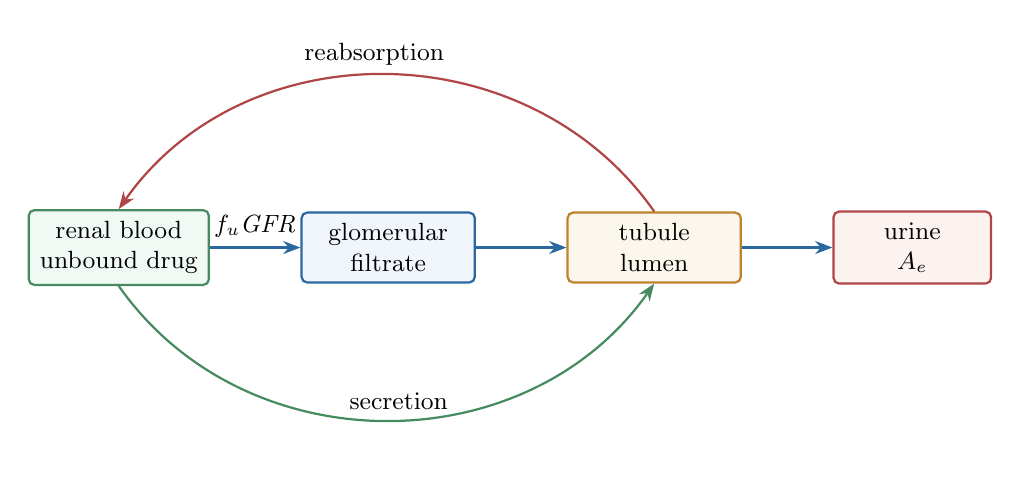
\begin{tikzpicture}[font=\small, node distance=.9cm and 1.15cm]
  \node[pkboxgreen, minimum width=2.2cm] (blood) {renal blood\\unbound drug};
  \node[pkbox, right=of blood, minimum width=2.2cm] (filtrate) {glomerular\\filtrate};
  \node[pkboxamber, right=of filtrate, minimum width=2.2cm] (tubule) {tubule\\lumen};
  \node[pkboxred, right=of tubule, minimum width=2.0cm] (urine) {urine\\\(A_e\)};
  \draw[pkarr] (blood) -- node[above] {\(f_u\pksym{GFR}\)} (filtrate);
  \draw[pkarr] (filtrate) -- (tubule);
  \draw[pkarr] (tubule) -- (urine);
  \draw[pkarrgreen] (blood.south) to[out=-55,in=-125,looseness=1.05]
    node[pos=.52, above] {secretion} (tubule.south);
  \draw[pkarrred] (tubule.north) to[out=125,in=55,looseness=1.05]
    node[pos=.52, above] {reabsorption} (blood.north);
\end{tikzpicture}%
}
\captionof{figure}{Renal clearance as filtration, secretion, and reabsorption. The drawing deliberately separates tubule lumen from blood so \(\pkCL_R\) can be read mechanistically.}
\end{center}
}

\newcommand{\figureTMDD}{
\begin{center}
\pkfitfigure{%
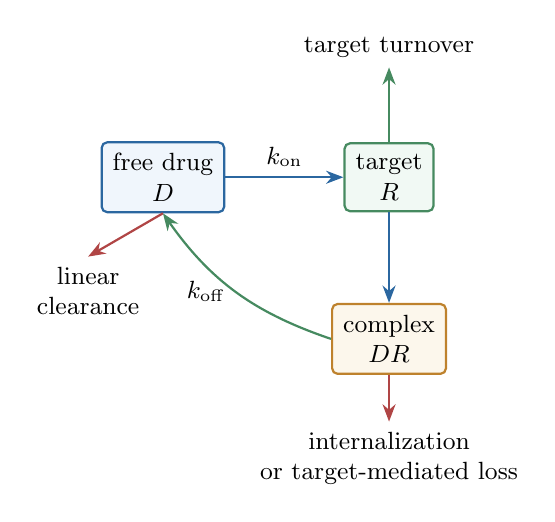
\begin{tikzpicture}[font=\small, node distance=1.0cm and 1.5cm]
  \node[pkbox] (drug) {free drug\\\(D\)};
  \node[pkboxgreen, right=of drug] (target) {target\\\(R\)};
  \node[pkboxamber, below=1.15cm of target] (complex) {complex\\\(DR\)};
  \draw[pkarr] (drug) -- node[above] {\(k_{\pklab{on}}\)} (target);
  \draw[pkarr] (target) -- (complex);
  \draw[pkarrgreen] (complex.west) to[bend left=18] node[left] {\(k_{\pklab{off}}\)} (drug.south);
  \draw[pkarrred] (complex) -- ++(0,-1.05) node[below,align=center] {internalization\\or target-mediated loss};
  \draw[pkarrred] (drug.south) -- ++(-.95,-.55) node[below,align=center] {linear\\clearance};
  \draw[pkarrgreen] (target.north) -- ++(0,.95) node[above] {target turnover};
\end{tikzpicture}%
}
\captionof{figure}{Target-mediated drug disposition. TMDD makes the pharmacological target part of the disposition model, so PK and PD become coupled rather than sequential.}
\end{center}
}

\newcommand{\figurePopPKHierarchy}{
\begin{center}
\pkfitfigure{%
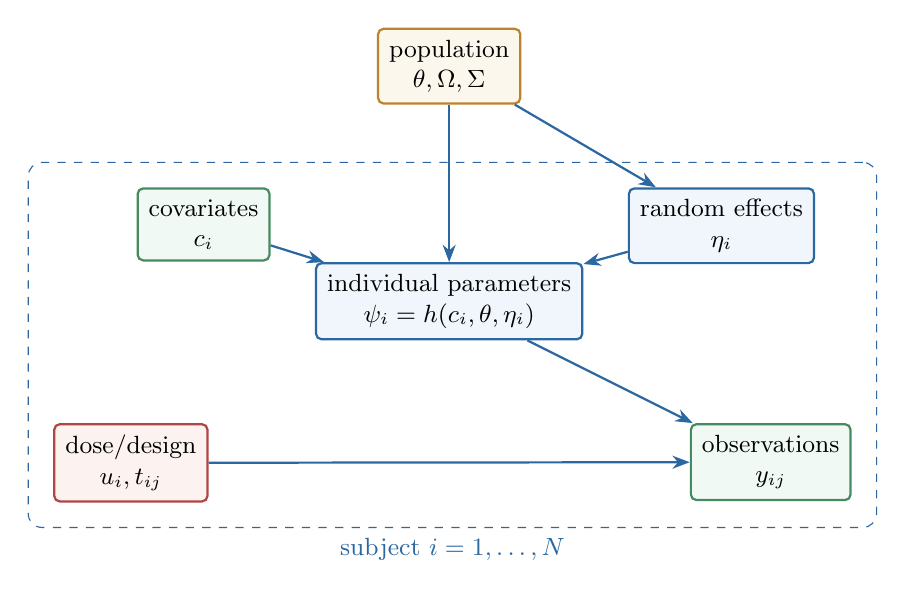
\begin{tikzpicture}[font=\small, node distance=1.05cm and 1.35cm]
  \node[pkboxamber] (theta) {population\\\(\theta,\Omega,\Sigma\)};
  \node[pkboxgreen, below left=of theta] (cov) {covariates\\\(c_i\)};
  \node[pkbox, below right=of theta] (eta) {random effects\\\(\eta_i\)};
  \node[pkbox, below=2.0cm of theta] (psi) {individual parameters\\\(\psi_i=h(c_i,\theta,\eta_i)\)};
  \node[pkboxred, below left=of psi] (dose) {dose/design\\\(u_i,t_{ij}\)};
  \node[pkboxgreen, below right=of psi] (obs) {observations\\\(y_{ij}\)};
  \draw[pkarr] (theta) -- (eta);
  \draw[pkarr] (theta) -- (psi);
  \draw[pkarr] (cov) -- (psi);
  \draw[pkarr] (eta) -- (psi);
  \draw[pkarr] (dose) -- (obs);
  \draw[pkarr] (psi) -- (obs);
  \node[draw=pkblue, dashed, rounded corners=5pt, fit=(cov)(eta)(psi)(dose)(obs), inner sep=9pt, label={[pkblue]below:subject \(i=1,\ldots,N\)}] {};
\end{tikzpicture}%
}
\captionof{figure}{Population PK hierarchy. NONMEM, SAEM, and Bayesian TDM are different computational cultures around this same latent-individual-parameter graph.}
\end{center}
}

\newcommand{\figurePBPK}{
\begin{center}
\pkfitfigure{%
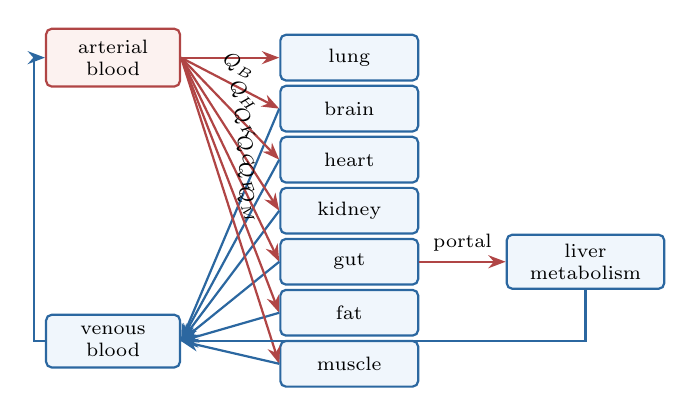
\begin{tikzpicture}[font=\scriptsize, x=1cm, y=.72cm]
  \node[pkboxred, minimum width=1.7cm] (art) at (0,5) {arterial\\blood};
  \node[pkbox, minimum width=1.7cm] (ven) at (0,0) {venous\\blood};
  \node[pkorgan] (lung) at (3.0,5.0) {lung};
  \node[pkorgan] (brain) at (3.0,4.1) {brain};
  \node[pkorgan] (heart) at (3.0,3.2) {heart};
  \node[pkorgan] (kidney) at (3.0,2.3) {kidney};
  \node[pkorgan] (gut) at (3.0,1.4) {gut};
  \node[pkorgan, minimum width=2.0cm] (liver) at (6.0,1.4) {liver\\metabolism};
  \node[pkorgan] (fat) at (3.0,.5) {fat};
  \node[pkorgan] (muscle) at (3.0,-.4) {muscle};
  \draw[pkarrred] (art) -- (lung);
  \foreach \o/\lab in {brain/\(Q_B\),heart/\(Q_H\),kidney/\(Q_K\),gut/\(Q_G\),fat/\(Q_F\),muscle/\(Q_M\)} {
    \draw[pkarrred] (art.east) -- node[above,sloped] {\lab} (\o.west);
    \draw[pkarr] (\o.west) -- (ven.east);
  }
  \draw[pkarrred] (gut) -- node[above] {portal} (liver);
  \draw[pkarr] (liver) |- (ven.east);
  \draw[pkarr] (ven) -- ++(-1,0) |- (art);
\end{tikzpicture}%
}
\captionof{figure}{A stripped-down PBPK circulation. Whole-body PBPK replaces abstract compartments with blood-flow-connected organs, while still preserving mass balance and observation maps.}
\end{center}
}

\newcommand{\figurePDDelays}{
\begin{center}
\pkfitfigure{%
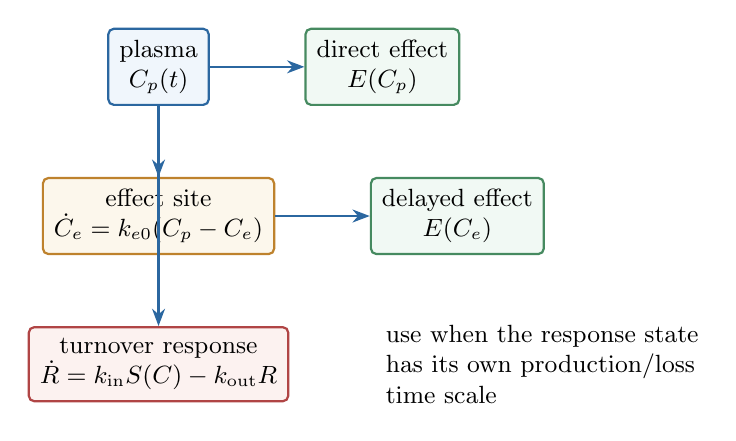
\begin{tikzpicture}[font=\small, node distance=.9cm and 1.2cm]
  \node[pkbox] (cp) {plasma\\\(C_p(t)\)};
  \node[pkboxgreen, right=of cp] (direct) {direct effect\\\(E(C_p)\)};
  \draw[pkarr] (cp) -- (direct);
  \node[pkboxamber, below=of cp] (ce) {effect site\\\(\dot C_e=k_{e0}(C_p-C_e)\)};
  \node[pkboxgreen, right=of ce] (effect) {delayed effect\\\(E(C_e)\)};
  \draw[pkarr] (cp) -- (ce);
  \draw[pkarr] (ce) -- (effect);
  \node[pkboxred, below=of ce, minimum width=3.1cm] (turn) {turnover response\\\(\dot R=k_{\pklab{in}}S(C)-k_{\pklab{out}}R\)};
  \draw[pkarr] (cp) -- (turn);
  \node[align=left, right=1.1cm of turn] {use when the response state\\has its own production/loss\\time scale};
\end{tikzpicture}%
}
\captionof{figure}{Three PD delay grammars. Direct effect, effect compartment, and turnover models answer different reasons why response and plasma concentration may disconnect.}
\end{center}
}

\newcommand{\figureStructureAbsorptionMap}{
\begin{center}
\pkfitfigure{%
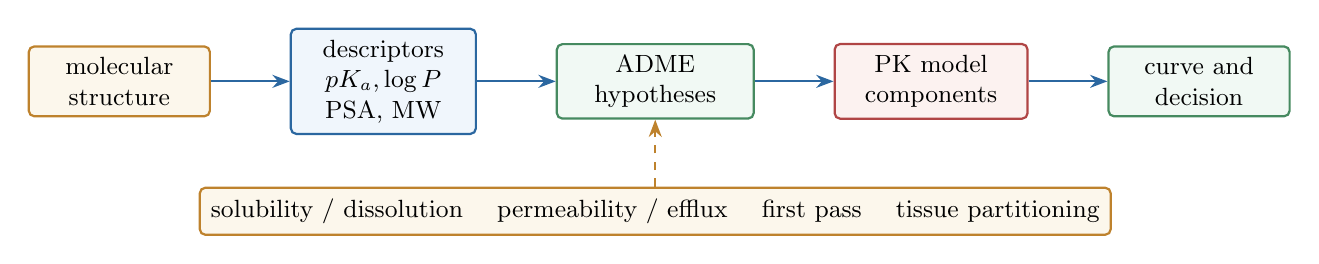
\begin{tikzpicture}[font=\small, node distance=.85cm and 1.0cm]
  \node[pkboxamber, minimum width=2.3cm] (mol) {molecular\\structure};
  \node[pkbox, right=of mol, minimum width=2.35cm] (desc) {descriptors\\\(pK_a,\log P\)\\PSA, MW};
  \node[pkboxgreen, right=of desc, minimum width=2.5cm] (hyp) {ADME\\hypotheses};
  \node[pkboxred, right=of hyp, minimum width=2.45cm] (model) {PK model\\components};
  \node[pkboxgreen, right=of model, minimum width=2.3cm] (data) {curve and\\decision};
  \draw[pkarr] (mol) -- (desc);
  \draw[pkarr] (desc) -- (hyp);
  \draw[pkarr] (hyp) -- (model);
  \draw[pkarr] (model) -- (data);
  \node[pkboxamber, below=of hyp, minimum width=6.6cm] (examples) {solubility / dissolution \quad permeability / efflux \quad first pass \quad tissue partitioning};
  \draw[pkdash] (examples) -- (hyp);
\end{tikzpicture}%
}
\captionof{figure}{Structure-PK as hypothesis generation. Molecular descriptors do not replace clinical data; they propose where to look in absorption, distribution, metabolism, excretion, and tissue exposure.}
\end{center}
}

\newcommand{\figureReversibleEhc}{
\begin{center}
\pkfitfigure{%
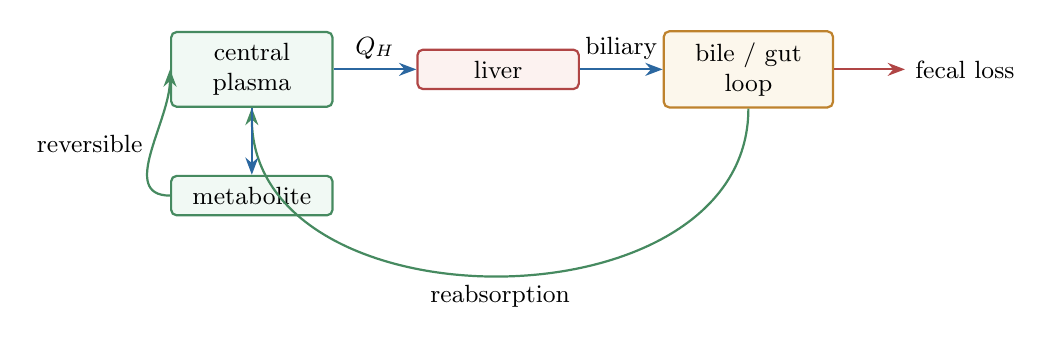
\begin{tikzpicture}[font=\small, node distance=.85cm and 1.05cm]
  \node[pkboxgreen, minimum width=2.05cm] (central) {central\\plasma};
  \node[pkboxred, right=of central, minimum width=2.05cm] (liver) {liver};
  \node[pkboxamber, right=of liver, minimum width=2.15cm] (bilegut) {bile / gut\\loop};
  \node[pkboxgreen, below=of central, minimum width=2.05cm] (met) {metabolite};
  \draw[pkarr] (central) -- node[above] {\(Q_H\)} (liver);
  \draw[pkarr] (liver) -- node[above] {biliary} (bilegut);
  \draw[pkarrgreen] (bilegut.south) to[out=-90,in=-90,looseness=1.15] node[pos=.5,below] {reabsorption} (central.south);
  \draw[pkarrred] (bilegut.east) -- ++(.9,0) node[right] {fecal loss};
  \draw[pkarr] (central) -- (met);
  \draw[pkarrgreen] (met.west) to[out=180,in=-90,looseness=1.05] node[pos=.55,left] {reversible} (central.west);
\end{tikzpicture}%
}
\captionof{figure}{Reversible systems and enterohepatic cycling. A secondary peak may be a real loop in the system, not merely noisy concentration data.}
\end{center}
}

\newcommand{\figureAdvancedPdDelayLadder}{
\begin{center}
\pkfitfigure{%
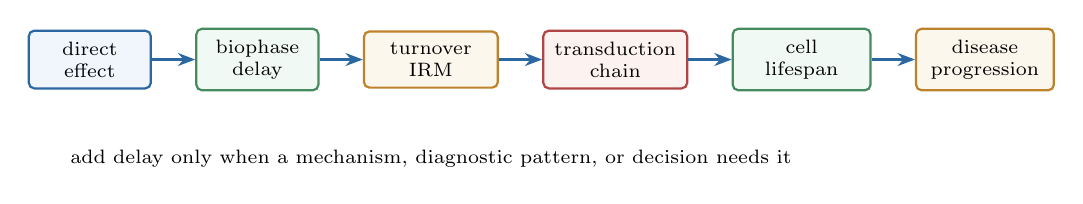
\begin{tikzpicture}[font=\scriptsize, node distance=.52cm and .55cm]
  \node[pkbox, minimum width=1.55cm] (direct) {direct\\effect};
  \node[pkboxgreen, right=of direct, minimum width=1.55cm] (bio) {biophase\\delay};
  \node[pkboxamber, right=of bio, minimum width=1.7cm] (turnover) {turnover\\IRM};
  \node[pkboxred, right=of turnover, minimum width=1.75cm] (trans) {transduction\\chain};
  \node[pkboxgreen, right=of trans, minimum width=1.75cm] (life) {cell\\lifespan};
  \node[pkboxamber, right=of life, minimum width=1.75cm] (disease) {disease\\progression};
  \draw[pkarr] (direct) -- (bio);
  \draw[pkarr] (bio) -- (turnover);
  \draw[pkarr] (turnover) -- (trans);
  \draw[pkarr] (trans) -- (life);
  \draw[pkarr] (life) -- (disease);
  \node[below=.65cm of turnover, align=center] {add delay only when a mechanism, diagnostic pattern, or decision needs it};
\end{tikzpicture}%
}
\captionof{figure}{The PHC 609 delay ladder. Advanced PD is not one model class; it is a disciplined escalation from immediate effect to biophase, turnover, transduction, cell lifespan, and disease dynamics.}
\end{center}
}

\newcommand{\figureQSPWorkflow}{
\begin{center}
\pkfitfigure{%
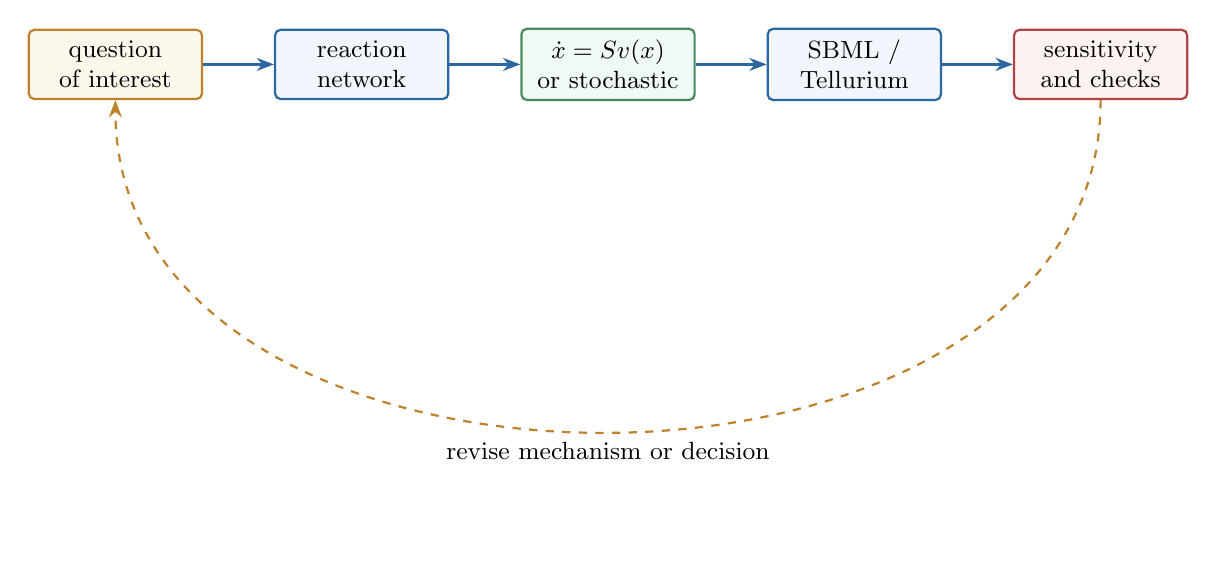
\begin{tikzpicture}[font=\small, node distance=.75cm and .9cm]
  \node[pkboxamber, minimum width=2.2cm] (q) {question\\of interest};
  \node[pkbox, right=of q, minimum width=2.2cm] (rxn) {reaction\\network};
  \node[pkboxgreen, right=of rxn, minimum width=2.2cm] (ode) {\(\dot x=Sv(x)\)\\or stochastic};
  \node[pkbox, right=of ode, minimum width=2.2cm] (sim) {SBML /\\Tellurium};
  \node[pkboxred, right=of sim, minimum width=2.2cm] (check) {sensitivity\\and checks};
  \draw[pkarr] (q) -- (rxn);
  \draw[pkarr] (rxn) -- (ode);
  \draw[pkarr] (ode) -- (sim);
  \draw[pkarr] (sim) -- (check);
  \draw[pkdash] (check.south) to[out=-90,in=-90,looseness=1.15] node[pos=.5,below] {revise mechanism or decision} (q.south);
\end{tikzpicture}%
}
\captionof{figure}{QSP implementation loop. A pathway diagram becomes useful when it is turned into equations, simulated reproducibly, stress-tested, and tied back to a decision.}
\end{center}
}

\emergencystretch=2em
\setcounter{tocdepth}{2}

\DeclareMathOperator{\Var}{Var}
\DeclareMathOperator{\Cov}{Cov}
\DeclareMathOperator{\diag}{diag}
\DeclareMathOperator{\logit}{logit}
\DeclareMathOperator*{\argmin}{arg\,min}
\DeclareMathOperator*{\argmax}{arg\,max}

\newcommand{\R}{\mathbb{R}}
\newcommand{\Prob}{\mathbb{P}}
\newcommand{\E}{\mathbb{E}}
\newcommand{\Normal}{\mathcal{N}}
\newcommand{\given}{\,|\,}
\newcommand{\rv}[1]{\mathsf{#1}}
\newcommand{\bs}[1]{\boldsymbol{#1}}
\newcommand{\rtheta}{\boldsymbol{\theta}}
\newcommand{\reta}{\boldsymbol{\eta}}
\newcommand{\repsilon}{\boldsymbol{\epsilon}}
\newcommand{\rpsi}{\boldsymbol{\psi}}
\newcommand{\data}{\mathcal{D}}
\newcommand{\loss}{\mathcal{L}}
\newcommand{\pkCL}{\pksym{CL}}
\newcommand{\pkV}{\pksym{V}}
\newcommand{\pkVc}{\pksym{V}_{c}}
\newcommand{\pkVss}{\pksym{V}_{ss}}
\newcommand{\pkF}{\pksym{F}}
\newcommand{\pkAUC}{\pksym{AUC}}
\newcommand{\pkAUMC}{\pksym{AUMC}}
\newcommand{\pkMRT}{\pksym{MRT}}
\newcommand{\pkCmax}{C_{\max}}
\newcommand{\pkTmax}{T_{\max}}
\newcommand{\pkCss}{C_{ss}}
\newcommand{\pkCavg}{C_{ss,\pklab{avg}}}
\newcommand{\pkCtrough}{C_{\pklab{trough}}}
\newcommand{\pkCpeak}{C_{\pklab{peak}}}
\newcommand{\pkka}{k_a}
\newcommand{\pkke}{k_e}
\newcommand{\pkQ}{\pksym{Q}}
\newcommand{\pkKm}{K_m}
\newcommand{\pkVmax}{V_{\max}}
\newcommand{\pkECfifty}{\pksym{EC}_{50}}
\newcommand{\pkICfifty}{\pksym{IC}_{50}}
\newcommand{\pkPD}{\pksym{PD}}
\newcommand{\pkPK}{\pksym{PK}}
\newcommand{\pkTMDD}{\pksym{TMDD}}
\newcommand{\pkPBPK}{\pksym{PBPK}}
\newcommand{\pkQSP}{\pksym{QSP}}
\newcommand{\pkNONMEM}{\pksym{NONMEM}}

\title{UB PHC 607/608/609 - Clinical PK/PD as Dose Individualization}

\begin{document}
\maketitle
{\small
  \noindent\textbf{Reading motive}\\
  这份笔记把 Buffalo PHC 607/608/609 相关材料重写成一卷完整的自学文本。Guohua An 的两本 notebook 给出课程的覆盖面：clinical pharmacokinetics, dose optimization, biologics, advanced PK/PD, PBPK, population PK, NONMEM, pharmacodynamics, indirect response, and QSP \cite{an2025essentialsClinicalPK,an2025advancedPKPD}. 这里不做逐句改写，也不做替代教材式复制；我把它们当作 topic map，然后用我们前面形成的 dec41/pdf2htmlEX 风格写成一条原创推理线。\hspace*{\fill}[source map]

  \vspace{5pt}
  \noindent\textbf{Audience}\\
  读者可以没有系统学过 PK/PD。全书从 dose, concentration, amount, clearance, volume, probability, and decision 开始，然后逐步走到 clinical dose adjustment, biologics, nonlinear kinetics, population PK, PBPK, PD, TMDD and QSP. 目标不是背参数，而是让读者知道一个临床剂量问题如何变成可计算、可解释、可质疑、可更新的模型问题。\hspace*{\fill}[from zero]

  \vspace{5pt}
  \noindent\textbf{Style}\\
  中英文混排。中文负责逻辑铺垫和判断，英文保留药动药效、模型和软件语境里最自然的术语。符号沿用我们之前的规则：random variables 用 sans-serif，Greek random quantities 用 bold Greek，多字母 PK/PD 固定搭配在数学公式中用 text italic label，比如 \(\pkCL,\pkAUC,\pkPK,\pkPD,\pkPBPK,\pkQSP\)。\hspace*{\fill}[notation]
}

\tableofcontents

\section{The Unifying Problem}

\subsection{Dose is not the object; decision is the object}

Clinical pharmacokinetics 常常从一句话开始：what the body does to the drug. 这句话没错，但它太静态。真正的课程主线应该是：
\[
  \text{dose}
  \longrightarrow
  \text{exposure}
  \longrightarrow
  \text{response}
  \longrightarrow
  \text{decision}
  \longrightarrow
  \text{next dose}.
\]
If dose were the object, the course would end after prescription. If exposure were the object, it would end after plotting concentration--time curves. But clinical PK/PD is a decision science: we ask how a dose should be chosen, adapted, delayed, held, escalated, de-escalated, or individualized under uncertainty.

This is why PHC 607/608/609 naturally form one book. PHC 607 names the objects: concentration, amount, absorption, distribution, clearance, bioavailability, half-life, and exposure. PHC 608 turns those objects into dosing operations: loading dose, maintenance dose, infusion, accumulation, fluctuation, nonlinear elimination, special populations, therapeutic drug monitoring. PHC 609 then asks what happens when the simple objects are no longer sufficient: advanced PK/PD, PBPK, population models, biologics, target-mediated disposition, indirect response, and QSP.

\subsection{The central equation}

The most compact form of the whole course is
\[
  p_\theta(y_i,\psi_i,r_i\given u_i,c_i)
  =
  p_\theta(r_i\given y_i,\psi_i,u_i,c_i)\,
  p_\theta(y_i\given \psi_i,u_i)\,
  p_\theta(\psi_i\given c_i).
\]
Here \(u_i\) is the dosing and sampling design, \(c_i\) is covariate information, \(\psi_i\) is individual physiology and pharmacology, \(y_i\) is observed data, and \(r_i\) is response or clinical outcome.  The first semester asks how \(u_i\) becomes \(y_i\).  The second asks how to use \(y_i\) to choose the next \(u_i\).  The third asks how to learn \(p_\theta\) from many patients and then use it responsibly.

\figureDecisionLoop

\begin{remark}
  Classical PK looks deterministic because many textbook equations are deterministic. Clinical PK is not deterministic. The deterministic equation is the forward map inside a larger uncertain system: uncertain patient, uncertain adherence, uncertain sampling time, uncertain assay, uncertain response, uncertain future.
\end{remark}

\subsection{What makes a clinical PK/PD mind}

A clinical PK/PD mind learns to ask five questions before touching software:
\begin{enumerate}[leftmargin=2em]
  \item What is the decision? Dose, schedule, label, trial design, mechanism, or prediction?
  \item What is observed? Concentration, urine amount, biomarker, response, toxicity, survival, or only sparse clinical data?
  \item What is latent? Individual \(\pkCL\), \(\pkV\), target expression, enzyme activity, adherence, effect-site concentration, or disease state?
  \item What is shared across patients? Typical values, variability, covariate effects, residual error, physiological constants, or mechanistic pathways?
  \item What would falsify the working model? Wrong slope, wrong peak, wrong trough, wrong variability, wrong delay, wrong dose-response, or wrong special-population prediction?
\end{enumerate}

The answer to these questions decides whether a one-compartment model is enough, whether NCA is the right summary, whether a well-stirred liver model is appropriate, whether a biologic needs TMDD, whether NONMEM is necessary, and whether a QSP model is credible.

\section{Notation and Symbol Discipline}

\subsection{Random variables and realized values}

We adopt the inference notation used in the earlier Bayesian PopPK note. A random concentration before observation is \(\rv{C}(t)\); an observed concentration is \(C(t)\). A random individual clearance is \(\rv{CL}_i\); a realized or candidate value is \(\pkCL_i\). Greek random quantities use bold Greek:
\[
  \reta_i \sim \Normal(0,\Omega),
  \qquad
  \repsilon_{ij}\sim\Normal(0,\sigma^2).
\]
This visual discipline matters because clinical PK constantly moves between population, individual, and observation.

\begin{center}
\begin{tabularx}{0.95\textwidth}{@{}lX@{}}
\toprule
Symbol & Meaning \\
\midrule
\(\rv{Y}_{ij}\) & random observation, for example a future concentration. \\
\(y_{ij}\) & observed value after the assay reports a number. \\
\(\rpsi_i\) & random individual parameter vector. \\
\(\psi_i\) & candidate or realized individual parameter value. \\
\(\theta\) & population parameter when treated as an unknown fixed quantity. \\
\(\rtheta\) & population parameter when treated as random in full Bayes. \\
\(\pkCL,\pkV,\pkAUC,\pkAUMC,\pkPK,\pkPD\) & fixed multi-letter PK/PD labels in equations. \\
\bottomrule
\end{tabularx}
\end{center}

\subsection{Primary and secondary parameters}

The course becomes clearer if we distinguish primary from secondary quantities. Primary parameters are closer to the system's mechanisms: \(\pkCL\), \(\pkV\), \(k_a\), bioavailability \(\pkF\), distribution clearance \(\pkQ\), binding fractions, intrinsic clearance, organ blood flow. Secondary quantities are derived from them:
\[
  t_{1/2}=\frac{\log 2}{\pkke},
  \qquad
  \pkke=\frac{\pkCL}{\pkV},
  \qquad
  \pkAUC=\frac{\pkF\,\pksym{Dose}}{\pkCL}.
\]
Half-life is not a knob in the body. It is the visible consequence of clearance and volume. The same half-life can arise from high \(\pkCL\) and high \(\pkV\), or from low \(\pkCL\) and low \(\pkV\). This is why dose adjustment by half-life alone is often crude.

\subsection{The four layers of a formula}

Every formula has four layers:
\begin{enumerate}[leftmargin=2em]
  \item algebraic layer: the symbols balance;
  \item unit layer: amount, volume, time, and concentration are consistent;
  \item physiological layer: the signs and dependencies make biological sense;
  \item decision layer: the equation answers the current clinical question.
\end{enumerate}
For example, \(\pkAUC=\pksym{Dose}/\pkCL\) is algebraically simple. But if the route is oral, the formula becomes \(\pkAUC=\pkF\pksym{Dose}/\pkCL\). If \(\pkCL\) is plasma clearance, organ extraction arguments require blood-to-plasma correction. If protein binding changes, total and unbound \(\pkAUC\) may tell different clinical stories. A beautiful formula can still be the wrong formula for the decision.

\section{PHC 607: The Concentration-Time Grammar}

\subsection{Amount, concentration, and compartments}

The first conceptual split is amount versus concentration. Amount \(A(t)\) is how much drug is in a compartment. Concentration \(C(t)\) is amount divided by a volume-like scaling:
\[
  C(t)=\frac{A(t)}{\pkV}.
\]
The volume is not necessarily an anatomic bucket. It is a proportionality that turns amount into the measured concentration in the sampled matrix. A large apparent volume of distribution does not mean the body has a giant physical container. It means plasma concentration is small relative to total amount.

Compartment models are bookkeeping devices for mass balance. A compartment is a region that is assumed to be kinetically homogeneous for the question at hand. It can represent plasma, central extracellular fluid, tissue, effect site, gut, liver, target binding, or a mathematical delay. The model is judged by whether its compartments create the right predictions, not by whether every compartment has a literal wall.

\figureCompartmentFamily

\subsection{The first mass-balance equation}

The one-compartment IV bolus model starts with
\[
  \frac{\dd A(t)}{\dd t}=-\pkke A(t),
  \qquad
  A(0)=\pksym{Dose}.
\]
The solution is
\[
  A(t)=\pksym{Dose}\,e^{-\pkke t},
  \qquad
  C(t)=C_0e^{-\pkke t},
  \qquad
  C_0=\frac{\pksym{Dose}}{\pkV}.
\]
This is the first clinical grammar: the intercept names distribution scale, the slope names elimination speed. But the intercept and slope are not independent mechanisms:
\[
  \pkCL=\pkke\pkV.
\]
The slope is not simply ``renal function'' or ``metabolism.'' It is clearance divided by volume.

\subsection{Zero-order and first-order as questions about rate}

First-order elimination says the rate is proportional to amount:
\[
  \frac{\dd A}{\dd t}=-kA.
\]
Zero-order elimination says the rate is approximately constant:
\[
  \frac{\dd A}{\dd t}=-R.
\]
The clinical meaning is not ``one is easy and one is hard.'' The clinical meaning is capacity. First-order kinetics is what a low-concentration approximation often looks like when elimination capacity is not stressed. Zero-order kinetics appears when the system is locally saturated or when input is controlled at a constant rate. PHC 609 will later reframe this using Michaelis--Menten elimination:
\[
  \frac{\dd A}{\dd t}
  =
  -\frac{\pkVmax C}{\pkKm+C}.
\]
When \(C\ll \pkKm\), the expression is approximately first-order; when \(C\gg \pkKm\), it is approximately zero-order.

\section{Clearance as the Main Invariant}

\subsection{Clearance is a proportionality, not a cleaned volume}

Clearance is defined by
\[
  \text{rate of elimination}=\pkCL\,C.
\]
The phrase ``volume cleared per time'' is useful but dangerous. No physical volume of plasma is necessarily scrubbed clean. Clearance is a proportionality between concentration and elimination rate. It is the parameter that lets exposure connect to dose:
\[
  \pkAUC_{0-\infty}=\frac{\pksym{Dose}}{\pkCL}
  \quad \text{for IV bolus with linear elimination}.
\]
If the drug is extravascular,
\[
  \pkAUC_{0-\infty}=\frac{\pkF\,\pksym{Dose}}{\pkCL}.
\]
Thus, for linear PK, exposure is mostly a clearance story. Volume shapes the time profile, but clearance controls total exposure.

\subsection{Systemic, organ, blood, plasma, and unbound clearance}

The first subtlety is reference concentration. A hepatic extraction model uses blood concentration entering and leaving the liver. Many clinical assays report plasma concentration. If \(C_b\) is blood concentration and \(C_p\) is plasma concentration, then
\[
  \pkCL_b = \pkCL_p\frac{C_p}{C_b}.
\]
Confusing plasma clearance with blood clearance can make a drug seem to exceed organ blood flow, not because physiology is impossible, but because the denominator changed.

The second subtlety is binding. For many mechanistic arguments, unbound concentration is closer to the concentration available for transport, metabolism, receptor binding, and filtration. Total concentration is what we often measure, but unbound concentration is often what the enzyme or target sees:
\[
  C_u=f_u C.
\]
The art is not to worship \(C_u\) blindly. The art is to ask which concentration the model equation is using.

\subsection{Extraction ratio}

Organ clearance can be written
\[
  \pkCL_{\pklab{organ}}=\pkQ\,E,
\]
where \(\pkQ\) is organ blood flow and \(E\) is extraction ratio. For liver,
\[
  E_H=\frac{C_{\pklab{in}}-C_{\pklab{out}}}{C_{\pklab{in}}},
  \qquad
  \pkCL_H=Q_H E_H.
\]
High-extraction drugs are flow sensitive: changing \(Q_H\) changes clearance strongly. Low-extraction drugs are capacity and binding sensitive: changing \(f_u\) or intrinsic clearance matters more. This is not a memorized classification; it follows from the well-stirred model,
\[
  \pkCL_H=\frac{Q_H f_u \pkCL_{\pklab{int}}}{Q_H+f_u \pkCL_{\pklab{int}}}.
\]
If \(f_u\pkCL_{\pklab{int}}\gg Q_H\), then \(\pkCL_H\approx Q_H\). If \(f_u\pkCL_{\pklab{int}}\ll Q_H\), then \(\pkCL_H\approx f_u\pkCL_{\pklab{int}}\).

\section{Volume of Distribution and the Geography of Amount}

\subsection{Volume is a scaling}

The apparent volume of distribution is
\[
  \pkV=\frac{A}{C}.
\]
The denominator is usually plasma or blood concentration. If a drug leaves plasma and partitions into tissues, plasma concentration can be small while total amount remains large, so \(\pkV\) becomes large. This makes \(\pkV\) a map of where amount hides relative to the sampled compartment.

The clinical use of \(\pkV\) is immediate:
\[
  \pksym{Loading\ Dose}
  =
  \frac{C_{\pklab{target}}\pkV}{\pkF}.
\]
Loading dose is a distribution problem. Maintenance dose is a clearance problem. This single distinction prevents a lot of clinical confusion.

\subsection{Protein binding does not have one universal consequence}

Suppose plasma protein binding decreases, so \(f_u\) increases. What happens? It depends. The unbound concentration may initially rise, but clearance and distribution may also change. For a low-extraction hepatically cleared drug, total clearance may increase roughly with \(f_u\). For a high-extraction drug, hepatic clearance may be flow limited and less sensitive to \(f_u\). For a drug with a narrow therapeutic index where unbound concentration drives toxicity, a change in total concentration may be misleading.

The correct question is therefore not ``does protein binding matter?'' but
\[
  \text{which concentration drives elimination, distribution, response, and measurement?}
\]
When these differ, total concentration becomes a shadow of several mechanisms.

\subsection{Distribution rate versus distribution extent}

Extent of distribution is about how much drug lives outside the sampled space at equilibrium. Rate of distribution is about how fast it gets there. A two-compartment model separates these:
\[
  \begin{aligned}
  \frac{\dd A_c}{\dd t}
  &=
  -(\pkCL+\pkQ)\frac{A_c}{\pkVc}
  +
  \pkQ\frac{A_p}{V_p},\\
  \frac{\dd A_p}{\dd t}
  &=
  \pkQ\frac{A_c}{\pkVc}
  -
  \pkQ\frac{A_p}{V_p}.
  \end{aligned}
\]
Here \(\pkQ\) is distribution clearance. It controls exchange rate, not systemic elimination. A drug can have a large peripheral volume but slow equilibration, creating early high plasma concentrations followed by a long distribution tail.

\section{Absorption and Bioavailability}

\subsection{Extent and rate are different questions}

Absorption asks two questions:
\[
  \text{how much gets in?}
  \qquad
  \text{how fast does it get in?}
\]
The first is extent, often summarized by bioavailability \(\pkF\). The second is rate, often summarized by \(k_a\), \(\pkTmax\), and \(\pkCmax\). A formulation can preserve \(\pkAUC\) while lowering \(\pkCmax\). Another can increase \(\pkCmax\) without changing total exposure. These are not cosmetic differences: toxicity, efficacy, and tolerability may depend on peak, trough, duration, or total exposure.

For first-order absorption into a one-compartment model,
\[
  C(t)=
  \frac{\pkF\,\pksym{Dose}\,k_a}{\pkV(k_a-k_e)}
  \left(e^{-k_e t}-e^{-k_a t}\right).
\]
The curve rises because input initially exceeds elimination. It peaks when input and output balance. It falls when absorption has mostly finished and elimination dominates.

\subsection{Bioavailability is a product of barriers}

For oral dosing,
\[
  \pkF = F_a F_G F_H,
\]
where \(F_a\) is fraction absorbed across the gut wall, \(F_G\) is fraction escaping gut metabolism or efflux loss, and \(F_H\) is fraction escaping hepatic first pass. This factorization is a conceptual map, not always a directly identifiable statistical model. A low oral \(\pkF\) could reflect solubility, permeability, degradation, transporter efflux, intestinal metabolism, hepatic extraction, or several together.

\figureAbsorptionBarriers

\subsection{Flip-flop kinetics}

Normally \(k_a>k_e\), so terminal decline reflects elimination. In flip-flop kinetics, \(k_a<k_e\), so terminal decline reflects absorption. The terminal slope is then not the elimination slope. This is a beautiful cautionary example: the same visual straight line on a semi-log plot can mean different mechanisms depending on model structure.

The clinical consequence is serious. If the observed terminal half-life after an oral depot formulation is actually absorption-limited, using it to infer elimination half-life may overestimate how long drug remains once input stops.

\section{Noncompartmental Analysis as Geometry}

\subsection{NCA describes the curve before explaining it}

Noncompartmental analysis is often introduced as model-free. Better: NCA is low-model geometry plus a terminal exponential assumption. It reads the concentration-time curve by area, peak, time of peak, terminal slope, and moments:
\[
  \pkAUC=\int_0^\infty C(t)\,\dd t,
  \qquad
  \pkAUMC=\int_0^\infty tC(t)\,\dd t,
  \qquad
  \pkMRT=\frac{\pkAUMC}{\pkAUC}.
\]
The observed portion uses trapezoids. The unobserved tail uses \(\lambda_z\):
\[
  \pkAUC_{0-\infty}
  =
  \pkAUC_{0-t_{\pklab{last}}}
  +
  \frac{C_{\pklab{last}}}{\lambda_z}.
\]
Thus, NCA is not free of assumptions. It assumes the terminal portion chosen for \(\lambda_z\) is meaningful.

\figureAucTrapezoids

\subsection{AUC, Cmax, Tmax answer different questions}

\(\pkAUC\) is total exposure. \(\pkCmax\) is peak intensity. \(\pkTmax\) is a rough timing summary. For bioequivalence, \(\pkAUC\) and \(\pkCmax\) often carry the central evidence because they summarize extent and peak. For clinical toxicity, trough may matter more than peak. For concentration-dependent antibiotics, peak-to-MIC or AUC-to-MIC may be decisive. For time-dependent antibiotics, time above MIC matters.

The same curve contains many summaries. NCA is useful because it gives neutral summaries before committing to a structural explanation.

\subsection{When NCA is enough and when it is not}

NCA is often enough for single-dose exposure comparison, bioavailability, bioequivalence, and descriptive Phase 1 summaries. It is not enough when we need to predict unobserved regimens, covariate effects, sparse clinical sampling, nonlinear kinetics, delayed response, or patient-specific Bayesian updating. The transition from PHC 607 to PHC 608 is exactly this transition: from describing a curve to designing a regimen.

\section{From Single Dose to Repeated Dosing}

\subsection{Superposition}

For linear systems, multiple dosing can be built by superposition. If \(C_1(t)\) is the concentration after one dose, then dosing every \(\tau\) hours gives
\[
  C_n(t)=\sum_{m=0}^{n-1} C_1(t-m\tau)
  \quad \text{for terms with }t-m\tau\ge 0.
\]
This is the mathematical reason why the first one-compartment curve is not a toy. Once linearity holds, it becomes a reusable impulse response.

\subsection{Accumulation and steady state}

For one-compartment IV bolus with first-order elimination, the accumulation factor is
\[
  R=\frac{1}{1-e^{-k_e\tau}}.
\]
Steady state is not a static concentration; it is a periodic pattern where each dosing interval repeats. Peaks, troughs, and average concentration stabilize:
\[
  \pkCavg=\frac{\pkF\,\pksym{Dose}}{\pkCL\,\tau}.
\]
Average steady-state concentration is a clearance result. Fluctuation is a half-life and dosing-interval result. This lets us separate two questions: how high is the average exposure, and how rough is the ride?

\figureMultipleDosing

\subsection{Time to steady state}

Time to steady state is governed by \(k_e\), not by dose. It takes about four to five half-lives to get close to steady state for linear first-order kinetics. Raising the maintenance dose raises the plateau; it does not make the system approach the plateau faster. A loading dose can jump the system near the desired amount because loading is a volume problem:
\[
  \pksym{LD}=\frac{C_{\pklab{target}}\pkV}{\pkF}.
\]
Maintenance is then a clearance problem:
\[
  \pksym{MD}/\tau=\frac{C_{\pklab{target}}\pkCL}{\pkF}.
\]

\section{Infusion as Controlled Input}

\subsection{Zero-order input with first-order elimination}

For constant infusion rate \(R_0\),
\[
  \frac{\dd A}{\dd t}=R_0-\pkke A.
\]
The solution during infusion is
\[
  C(t)=\frac{R_0}{\pkCL}\left(1-e^{-\pkke t}\right).
\]
The steady-state concentration is
\[
  \pkCss=\frac{R_0}{\pkCL}.
\]
This is one of the cleanest clinical equations in PK. If target concentration is known and clearance is known, rate follows directly:
\[
  R_0=\pkCss\pkCL.
\]

\subsection{Stopping the infusion}

If infusion stops at time \(T\), concentration declines from whatever level was reached:
\[
  C(t)=C(T)e^{-\pkke(t-T)},\qquad t\ge T.
\]
This simple piecewise thinking is a major clinical skill. During infusion, input and elimination both act. After infusion, elimination acts alone. The equation you use depends on where the patient is in the regimen.

\subsection{Short infusions}

Many clinical regimens are neither bolus nor continuous infusion. A short infusion is a controlled input over a finite duration, repeated every \(\tau\). It combines the infusion rise and post-infusion decline. The important habit is to label the clock: time since start of infusion, time since end of infusion, and time within the dosing interval are not the same.

\section{Two-Compartment Thinking}

\subsection{Why biexponential curves happen}

After IV bolus, many drugs show a fast early decline and slower later decline:
\[
  C(t)=Ae^{-\alpha t}+Be^{-\beta t}.
\]
The fast phase is not necessarily rapid elimination. It may be distribution out of central compartment. The slow phase is not necessarily a separate depot. It is the terminal eigenmode of the coupled system.

This is where linear algebra quietly enters clinical PK. The exponents \(\alpha,\beta\) are macro-rate constants arising from the eigenvalues of the compartment system. The micro-rate constants \(k_{12},k_{21},k_{10}\) describe exchange and elimination. The observed curve is a mixture of modes.

\subsection{Volumes in a two-compartment world}

Several volumes appear:
\[
  \pkVc,\qquad
  \pkVss,\qquad
  V_\beta.
\]
\(\pkVc\) is the central volume relevant to initial concentration after IV bolus. \(\pkVss\) is the steady-state extent of distribution. \(V_\beta\) connects clearance to terminal slope:
\[
  V_\beta=\frac{\pkCL}{\beta}.
\]
These volumes answer different questions. Using the wrong one can distort loading dose, half-life interpretation, or tissue accumulation intuition.

\subsection{Central versus peripheral site of action}

If the site of action is central, early concentration matters. If the site of action is peripheral, effect may lag behind plasma concentration because peripheral equilibration is slow. This is one reason PK/PD cannot stop at plasma curves. A clinically relevant response may be driven by an effect-site concentration, receptor occupancy, cell turnover, or downstream biomarker.

\section{Metabolites and Sequential Systems}

\subsection{Parent to metabolite}

For a parent drug \(A_p\) forming a metabolite \(A_m\),
\[
  \frac{\dd A_p}{\dd t}=-k_pA_p,
  \qquad
  \frac{\dd A_m}{\dd t}=f_mk_pA_p-k_mA_m.
\]
The metabolite curve rises while formation exceeds elimination and falls when formation can no longer sustain it. If \(k_m\gg k_p\), metabolite kinetics are formation-rate limited. If \(k_p\gg k_m\), they are metabolite-elimination limited.

\subsection{Active metabolites}

An active metabolite changes the dose-response story. The parent concentration may fall while pharmacological activity persists. A response model may need parent, metabolite, or both:
\[
  E(t)=E_0+
  \frac{\Emax C_p(t)}{\pkECfifty+C_p(t)}
  +
  \frac{\Emax^m C_m(t)}{\pkECfifty^m+C_m(t)}.
\]
This is a simple formula, but it carries a clinical warning: measuring only parent may miss part of pharmacology.

\section{Nonlinear Pharmacokinetics}

\subsection{Symptoms of nonlinearity}

Nonlinear PK appears when dose changes do not produce proportional exposure:
\[
  \frac{\pkAUC_2}{\pkAUC_1}\ne
  \frac{\pksym{Dose}_2}{\pksym{Dose}_1}.
\]
Other symptoms include dose-dependent half-life, clearance changing with concentration, time-dependent kinetics, unexpected accumulation, and terminal slopes that change across doses.

Nonlinearity is not a moral failure of a model. It is often a biological clue: saturable absorption, solubility limit, saturable first-pass metabolism, capacity-limited elimination, saturable plasma or tissue binding, transporter saturation, target-mediated disposition, autoinduction, autoinhibition, or disease-modulated physiology.

\subsection{Michaelis--Menten elimination}

For capacity-limited elimination,
\[
  \frac{\dd A}{\dd t}
  =
  -\frac{\pkVmax C}{\pkKm+C}.
\]
The apparent clearance is
\[
  \pkCL_{\pklab{app}}(C)=\frac{\pkVmax}{\pkKm+C}.
\]
As concentration increases, apparent clearance decreases. This is why a small dose increase can produce a large concentration increase near saturation.

\subsection{Phenytoin as a clinical warning}

Phenytoin is a standard teaching example because it makes the clinical danger visible. At steady state,
\[
  R_{\pklab{in}}=\frac{\pkVmax C_{ss}}{\pkKm+C_{ss}}.
\]
Solving for \(C_{ss}\),
\[
  C_{ss}
  =
  \frac{\pkKm R_{\pklab{in}}}{\pkVmax-R_{\pklab{in}}}.
\]
If \(R_{\pklab{in}}\) approaches \(\pkVmax\), concentration climbs sharply. The denominator is the danger. Linear dose adjustment fails because there is no constant clearance.

\section{Therapeutic Drug Monitoring}

\subsection{TDM as Bayesian updating before software}

Therapeutic drug monitoring is often taught as plug-in equations. But the deeper logic is Bayesian:
\[
  \text{prior patient expectation}
  +
  \text{measured concentration}
  \longrightarrow
  \text{updated individual parameters}
  \longrightarrow
  \text{next dose}.
\]
Even a simple peak/trough aminoglycoside calculation implicitly combines prior model structure with observed data. Modern Bayesian TDM simply makes the hierarchy explicit.

\subsection{Peak, trough, AUC, and target}

Different drugs ask for different monitoring targets. Aminoglycosides may emphasize peak-to-MIC and trough safety. Vancomycin increasingly emphasizes AUC-guided dosing. Antiepileptics may use trough ranges, but interpretation depends on adherence, timing, protein binding, interacting drugs, and symptoms. Immunosuppressants require exposure control under substantial variability.

The correct TDM question is not ``is the level in range?'' It is:
\[
  \text{given this level, timing, dose history, patient physiology, and target, what should happen next?}
\]

\subsection{Measurement is part of the model}

Assay error, sampling time error, missed doses, infusion timing, and documentation errors can dominate the apparent PK story. A concentration drawn during distribution may not represent trough. A sample labeled as trough may have been drawn early. A patient may have missed a dose. The clinical model includes the hospital workflow.

\section{Special Populations}

\subsection{Pediatrics}

Pediatric dosing is not adult dosing divided by body weight. Maturation changes renal function, hepatic enzymes, plasma proteins, body water, fat fraction, gastric pH, gastric emptying, and blood flow. Size matters, but maturation matters too. A common population model separates them:
\[
  \pkCL_i
  =
  \pkCL_{\pklab{adult}}
  \left(\frac{\pksym{WT}_i}{70}\right)^{0.75}
  \pksym{Mat}(\pksym{PMA}_i)
  e^{\eta_{\pkCL,i}}.
\]
The allometric exponent captures size scaling; the maturation function captures developmental physiology.

\subsection{Elderly patients}

Elderly patients challenge single-parameter thinking. Renal function may decline, hepatic blood flow may change, body composition shifts, albumin may be lower, comedications increase, homeostatic reserve declines, and pharmacodynamic sensitivity may increase. A normal concentration can still be clinically excessive if response sensitivity changed.

\subsection{Obesity}

Obesity forces the distinction between loading and maintenance. Loading dose depends on distribution; maintenance dose depends on clearance. Total body weight, ideal body weight, adjusted body weight, lean body weight, and body surface area are not interchangeable. The right body-size descriptor depends on whether the drug distributes into adipose, lean tissue, extracellular water, or a mixture.

\subsection{Renal and hepatic impairment}

Renal impairment affects filtration, secretion, reabsorption, protein binding, metabolites, and sometimes nonrenal clearance through uremic effects on enzymes and transporters. Hepatic impairment affects blood flow, intrinsic clearance, protein binding, biliary excretion, shunting, and first-pass extraction. Dose adjustment cannot be reduced to one lab value, although creatinine clearance, eGFR, Child--Pugh, bilirubin, albumin, INR, and disease context are useful summaries.

\section{Drug-Drug Interactions}

\subsection{Enzymes, transporters, and exposure}

A drug-drug interaction is a change in the system map. Inhibition decreases a pathway's capacity. Induction increases expression or activity over time. Transporter inhibition can alter absorption, hepatic uptake, renal secretion, brain entry, or biliary excretion. The exposure consequence depends on fraction affected:
\[
  \frac{\pkAUC_{\pklab{with}}}{\pkAUC_{\pklab{without}}}
  \approx
  \frac{1}{(1-f_m)+f_m/R},
\]
where \(f_m\) is fraction of clearance through the pathway and \(R\) is the residual activity ratio. If a pathway contributes little, even strong inhibition may have modest effect. If a pathway dominates, modest inhibition may matter.

\subsection{Time course of interaction}

Not all interactions appear immediately. Competitive inhibition can be rapid. Mechanism-based inhibition may develop as enzyme is inactivated. Induction requires synthesis and degradation dynamics. Thus, the time course of interaction can be a PK/PD model of enzyme activity:
\[
  \frac{\dd E_{\pklab{enz}}}{\dd t}
  =
  k_{\pklab{syn}}(1+\pksym{Ind}(C))
  -
  k_{\pklab{deg}}E_{\pklab{enz}}.
\]
The observed drug concentration is downstream of this enzyme state.

\section{Biologics: A Different PK Intuition}

\subsection{Small molecules and biologics differ in scale}

Biologics are not merely large small molecules. Size, structure, route, target binding, proteolysis, FcRn recycling, immunogenicity, and tissue access create different PK intuitions. Oral absorption is usually not the default. Distribution may be limited by convection, neonatal Fc receptor recycling, binding, and tissue penetration. Clearance may involve proteolysis, target-mediated elimination, immune complexes, or cellular processing rather than CYP metabolism.

\subsection{Antibodies}

Monoclonal antibodies often have small central volumes, slow distribution, long half-lives, and nonlinear clearance at low concentrations when target-mediated elimination is important. FcRn recycling protects IgG from lysosomal degradation and contributes to long persistence. But target binding can create nonlinear elimination:
\[
  D+R
  \underset{k_{\pklab{off}}}{\overset{k_{\pklab{on}}}{\rightleftharpoons}}
  DR
  \xrightarrow{k_{\pklab{int}}}
  \varnothing.
\]
At low doses, target-mediated clearance can dominate. At high doses, target pathways saturate and nonspecific clearance may dominate.

\subsection{ADCs}

Antibody-drug conjugates are systems, not single molecules. The measured analyte might be conjugated antibody, total antibody, free payload, released payload metabolite, or antigen-bound complex. Linker stability, drug-antibody ratio, antigen expression, internalization, payload permeability, bystander killing, and off-target toxicity all matter. A single concentration curve can hide multiple chemical and biological entities.

\subsection{Oligonucleotides and cell therapies}

ASOs, siRNAs, and cell therapies further stretch standard PK. Oligonucleotides involve tissue uptake, endosomal escape, chemical modification, protein binding, renal handling, and long tissue residence. CAR-T therapies expand, contract, persist, traffic, and respond to antigen. Their ``PK'' may be cell count or vector copies, and their ``dose'' may start a living dynamical system.

\section{PHC 609: The Advanced Modeling Turn}

\subsection{Model of system versus model of data}

An advanced PK/PD course becomes easier when we separate model of system from model of data. A system model says how amounts, concentrations, receptors, biomarkers, cells, or disease states evolve. A data model says how observations are generated from those latent states:
\[
  \begin{aligned}
  \frac{\dd x}{\dd t} &= f(x,u,\psi,t),\\
  y_{ij} &= g(x(t_{ij}),\psi)+\epsilon_{ij}.
  \end{aligned}
\]
The first line is biology and pharmacology. The second is measurement. Confusing them leads to poor model criticism.

\subsection{Laplace transforms and SHAM}

For linear time-invariant PK systems, Laplace transforms reveal how input becomes output:
\[
  X(s)=G(s)U(s).
\]
Poles determine slopes. Gains determine heights and areas. The SHAM mnemonic -- slope, height, area, moment -- is a way to inspect curves without forgetting the system behind them. A concentration profile is not only a graph; it is a compressed signature of rate constants, volumes, clearance, input, and observation.

\subsection{Numerical solution is not a fallback}

Closed forms are pedagogically beautiful, but numerical ODE solution is not second-class. PBPK, TMDD, QSP, nonlinear PD, disease progression, and complex dosing histories usually require numerical integration. The key is not whether the solution is analytical; the key is whether the model is verified, identifiable enough for the question, and numerically stable under the scenarios used for decision.

\section{Fitting PK Models}

\subsection{Objective functions}

Fitting means choosing parameters whose predictions are close to data under a stated error model. Ordinary least squares assumes constant additive variance:
\[
  \min_\psi \sum_j (y_j-\hat y_j(\psi))^2.
\]
Weighted least squares accounts for changing variance:
\[
  \min_\psi \sum_j w_j(y_j-\hat y_j(\psi))^2.
\]
A likelihood-based approach writes the observation law explicitly:
\[
  y_j\given \psi\sim \Normal(\hat y_j(\psi),\sigma^2_j).
\]
The likelihood is not a technicality. It is the model of how assays, residual variability, and misspecification create discrepancies.

\subsection{Residual error models}

Common residual models include additive,
\[
  y=\hat y+\epsilon,
\]
proportional,
\[
  y=\hat y(1+\epsilon),
\]
and combined forms. On the log scale, multiplicative error becomes additive:
\[
  \log y=\log \hat y+\epsilon.
\]
Choosing the residual model changes which deviations are treated as surprising. This is why residual plots are not decorative; they are direct checks of the observation model.

\subsection{Local minima and parameter correlation}

PK model fitting often has correlated parameters. \(\pkCL\) and \(\pkV\) can compensate through half-life; \(k_a\) and \(k_e\) can trade off when absorption is poorly sampled; \(V_{\max}\) and \(K_m\) can be weakly identified outside the concentration range that tests saturation. A best fit can be numerically precise but scientifically fragile. Standard errors, profiles, bootstrap, posterior samples, and simulation checks all ask whether the fitted parameter is actually learned.

\section{Population Pharmacokinetics}

\subsection{The hierarchy}

Population PK begins when individual parameters vary:
\[
  \psi_i = h(c_i,\theta,\eta_i),
  \qquad
  \eta_i\sim\Normal(0,\Omega).
\]
A typical lognormal clearance model is
\[
  \pkCL_i
  =
  \theta_{\pkCL}
  \left(\frac{\pksym{WT}_i}{70}\right)^{\theta_{\pklab{WT}}}
  e^{\eta_{\pkCL,i}}.
\]
The observation model might be
\[
  y_{ij}
  =
  \hat y(t_{ij};\psi_i,u_i)(1+\epsilon_{ij}).
\]
This is the same hierarchy from the earlier Bayesian PopPK note, now placed inside the clinical PK/PD course.

\figurePopPKHierarchy

\subsection{Fixed effects, random effects, residual effects}

Fixed effects describe typical values and covariate relationships. Random effects describe unexplained interindividual variability. Residual effects describe observation-level mismatch. The three are not interchangeable. If a covariate is omitted, random variability may inflate. If a structural model is wrong, residual error may inflate. If data are sparse, individual random effects may shrink toward zero. Diagnostics must ask which layer is absorbing the mismatch.

\subsection{NONMEM as an inference dialect}

NONMEM's \(\pklab{THETA}\), \(\pklab{ETA}\), and \(\pklab{EPS}\) syntax is not a separate theory. It is a dialect for the hierarchy:
\[
  \begin{array}{lll}
  \pklab{THETA} &\leftrightarrow& \text{population typical values and covariate effects},\\
  \pklab{ETA} &\leftrightarrow& \text{individual deviations},\\
  \pklab{EPS} &\leftrightarrow& \text{residual observation noise},\\
  \Omega,\Sigma &\leftrightarrow& \text{variance components}.
  \end{array}
\]
The objective function approximates a marginal likelihood where individual random effects have been integrated out. FO, FOCE, Laplacian, SAEM, and MCMC are different computational routes through the same conceptual problem.

\section{Bayesian Dose Individualization}

\subsection{Individual posterior}

Given a population model and a patient's observed concentrations,
\[
  p(\psi_i\given y_i,c_i,u_i,\theta)
  \propto
  p(y_i\given \psi_i,u_i)
  p(\psi_i\given c_i,\theta).
\]
This is the mathematical heart of Bayesian TDM. The prior-like term is the population model. The likelihood is the patient's measured data. The posterior is the updated individual PK state.

\subsection{Decision rule}

The dose is not chosen from a point estimate alone. In principle, the next regimen \(a\) should minimize expected loss:
\[
  a^*
  =
  \argmin_a
  \E\left[
    \loss(a,\tilde y,\tilde r)
    \given y_i,c_i,u_i
  \right].
\]
Here \(\tilde y\) and \(\tilde r\) are future exposure and response. A trough target, AUC target, toxicity constraint, or probability-of-target-attainment rule is a practical version of this expected-loss calculation.

\subsection{Why posterior uncertainty matters}

Two patients may have the same posterior mean \(\pkCL\) but different uncertainty. A robust dosing decision may differ if one posterior is tight and the other is broad. Sparse sampling, uncertain adherence, renal instability, rapidly changing disease, and nonlinear kinetics widen the posterior predictive distribution. A good Bayesian report should show not only the recommended dose but also the uncertainty in achieving the target.

\section{PBPK: Physiology as Model Architecture}

\subsection{Whole-body structure}

PBPK models replace abstract compartments with physiological tissues connected by blood flow:
\[
  \frac{\dd A_j}{\dd t}
  =
  Q_j C_{\pklab{art}}
  -
  Q_j\frac{C_j}{K_{p,j}}
  -
  \pksym{Elim}_j.
\]
The parameters now include tissue volumes, blood flows, partition coefficients, permeability, enzyme abundances, transporter activities, plasma binding, and route-specific absorption physiology.

\figurePBPK

\subsection{What PBPK is good for}

PBPK is especially useful when extrapolation depends on physiology: first-in-human translation, pediatric scaling, pregnancy, renal/hepatic impairment, drug-drug interactions, tissue exposure, transporter hypotheses, and virtual populations. Its power is not that it has many compartments. Its power is that those compartments are anchored to measurable physiological quantities.

\subsection{What PBPK is not}

PBPK is not automatically more true because it is more detailed. A complex model can hide uncertainty behind many parameters. The key questions are:
\[
  \text{which prediction is needed, which parameters control it, and what evidence supports those parameters?}
\]
This is the same discipline as simpler PK, only with more moving parts.

\section{Target-Mediated Drug Disposition}

\subsection{The basic mechanism}

TMDD occurs when binding to a pharmacological target changes disposition. A minimal model is
\[
  \begin{aligned}
  \frac{\dd D}{\dd t}
  &=
  -k_{\pklab{on}}DR+k_{\pklab{off}}DR_c-\pkCL_{\pklab{lin}}D,\\
  \frac{\dd R}{\dd t}
  &=
  k_{\pklab{syn}}-k_{\pklab{deg}}R
  -k_{\pklab{on}}DR+k_{\pklab{off}}DR_c,\\
  \frac{\dd DR_c}{\dd t}
  &=
  k_{\pklab{on}}DR-(k_{\pklab{off}}+k_{\pklab{int}})DR_c.
  \end{aligned}
\]
This model links PK and pharmacology because the target is both a sink and a mediator of effect.

\figureTMDD

\subsection{Small molecule versus large molecule TMDD}

For biologics, TMDD often appears because target binding and internalization are important relative to nonspecific clearance. For small molecules, target binding may be rapid, tissue-localized, or not a major elimination route, so TMDD may be harder to see or mechanistically different. The visual symptom -- nonlinear exposure -- is not enough. We need mechanism, target biology, concentration range, and perturbation evidence.

\subsection{Reduced TMDD models}

Full TMDD models can be difficult to identify. Quasi-equilibrium and quasi-steady-state approximations reduce the system when binding dynamics are fast relative to disposition. These approximations are not shortcuts by laziness; they are scientific statements about time scales. If the time-scale statement is wrong, the reduced model can mislead.

\section{Pharmacodynamics}

\subsection{Direct effect}

The simplest PD model maps concentration to effect immediately:
\[
  E(C)=E_0+\frac{\Emax C}{\pkECfifty+C}.
\]
The direct-effect model is appropriate when measured concentration equilibrates rapidly with the biophase and response is immediate. It teaches three ideas: baseline, maximum effect, and potency. But many clinical responses are not immediate.

\subsection{Effect compartment}

When plasma concentration and effect show hysteresis, an effect compartment can introduce equilibration delay:
\[
  \frac{\dd C_e}{\dd t}=k_{e0}(C_p-C_e),
  \qquad
  E(t)=E(C_e(t)).
\]
The effect compartment is not necessarily a physical compartment. It is a kinetic representation of delay between measured concentration and biophase concentration.

\subsection{Indirect response}

If drug changes production or loss of a response variable, an indirect response model is more natural:
\[
  \frac{\dd R}{\dd t}
  =
  k_{\pklab{in}}\,S(C)
  -
  k_{\pklab{out}}R
\]
or
\[
  \frac{\dd R}{\dd t}
  =
  k_{\pklab{in}}
  -
  k_{\pklab{out}}\,I(C)R.
\]
This class explains delayed onset, rebound, tolerance-like behavior, and biomarker turnover. The response time scale is now governed by \(k_{\pklab{out}}\), not only by drug half-life.

\figurePDDelays

\section{Exposure-Response and Clinical Development}

\subsection{Learning versus confirming}

Clinical development alternates between learning and confirming. Early studies learn tolerability, PK, dose range, and target engagement. Middle studies learn exposure-response and select dose. Pivotal studies confirm benefit-risk. Exposure-response analysis prevents dose selection from becoming a ritual of pairwise dose comparisons.

\subsection{Dose selection}

The dose should be justified by a chain:
\[
  \text{dose}
  \to
  \text{exposure}
  \to
  \text{target engagement}
  \to
  \text{biomarker}
  \to
  \text{clinical response}
  \to
  \text{safety}.
\]
Not every program has every link. But the missing links should be named. Model-informed drug development is disciplined storytelling with equations, not curve fitting for decoration.

\subsection{Project Optimus and oncology}

Oncology historically tolerated maximum tolerated dose logic, especially for cytotoxic agents. Targeted therapies and immunotherapies often require more nuanced dose optimization. If efficacy saturates before toxicity, the highest tolerated dose may not be the best dose. PK/PD and exposure-response become central to choosing a dose that balances activity, tolerability, adherence, and long-term benefit.

\section{QSP and Systems Pharmacology}

\subsection{When PK/PD becomes a system}

QSP appears when the response cannot be represented by one turnover variable or one effect-site delay. Immune cells, cytokines, tumor burden, receptor trafficking, signaling networks, feedback loops, and disease progression may all interact. The state vector becomes
\[
  \frac{\dd x}{\dd t}=f(x,u,\theta,t),
  \qquad
  y=g(x,\theta,t)+\epsilon.
\]
PK is one part of the state system, not the whole model.

\subsection{Platform models}

Platform QSP models try to reuse a mechanistic scaffold across related drugs or targets: bispecific antibodies, ADCs, siRNAs, immuno-oncology combinations. The promise is learning across programs. The danger is carrying forward assumptions beyond their evidence. Reuse is powerful only when assumptions travel with uncertainty.

\subsection{Credibility}

A QSP model is credible relative to a question of interest. It is not globally credible. For dose selection, the model must be credible for exposure-response in the relevant population and dose range. For mechanism exploration, qualitative dynamics may suffice. For regulatory support, documentation, verification, validation, sensitivity analysis, and uncertainty quantification become part of the model itself.

\section{A Three-Course Learning Route}

\subsection{PHC 607: name the objects}

Start by learning to read a concentration-time curve:
\[
  \pkCmax,\quad \pkTmax,\quad \pkAUC,\quad \lambda_z,\quad t_{1/2},\quad \pkCL,\quad \pkV,\quad \pkF.
\]
Then attach those summaries to LADME: liberation, absorption, distribution, metabolism, excretion. Do not rush to software. Learn what a slope means, what an intercept means, what area means, what a moment means, and what units reveal.

\subsection{PHC 608: design the regimen}

Next, learn to use the objects:
\[
  \pksym{LD}=\frac{C_{\pklab{target}}\pkV}{\pkF},
  \qquad
  \pksym{MD}/\tau=\frac{C_{\pklab{target}}\pkCL}{\pkF}.
\]
Study multiple dosing, infusion, oral absorption, two-compartment kinetics, nonlinear elimination, special populations, TDM, and drug interactions. The guiding question is always: what would I change in the next regimen, and why?

\subsection{PHC 609: build and criticize models}

Finally, learn model-based pharmacology:
\[
  \text{ODE}
  \to
  \text{likelihood}
  \to
  \text{population hierarchy}
  \to
  \text{prediction}
  \to
  \text{model criticism}.
\]
This includes numerical integration, fitting, nonlinear PK, PBPK, PopPK, NONMEM, Bayesian updating, TMDD, direct and indirect PD, exposure-response, and QSP. The goal is not complexity. The goal is choosing the simplest model that can support the decision without hiding the important uncertainty.

\section{Worked Mini-Cases}

\subsection{Case 1: loading and maintenance}

A patient needs rapid achievement of a target concentration \(C^*\). The model suggests \(\pkV=40\ \pksym{L}\), \(\pkCL=5\ \pksym{L/h}\), and \(\pkF=1\). The loading dose is
\[
  \pksym{LD}=C^*\pkV.
\]
The maintenance infusion rate is
\[
  R_0=C^*\pkCL.
\]
If \(\pkV\) doubles but \(\pkCL\) is unchanged, the loading dose doubles while maintenance rate remains the same. If \(\pkCL\) doubles but \(\pkV\) is unchanged, maintenance rate doubles while loading dose remains the same. This is the cleanest way to separate distribution from elimination.

\subsection{Case 2: oral exposure falls}

Suppose oral \(\pkAUC\) falls after coadministration with another drug. The equation
\[
  \pkAUC=\frac{F_aF_GF_H\,\pksym{Dose}}{\pkCL}
\]
creates hypotheses: reduced dissolution, reduced permeability, increased efflux, induced gut metabolism, induced hepatic metabolism, increased systemic clearance, or adherence/timing error. The curve shape helps prioritize. Lower \(\pkCmax\) with similar terminal slope suggests absorption or bioavailability. Lower exposure with changed terminal slope may suggest systemic clearance.

\subsection{Case 3: sparse TDM}

A patient has one concentration after several doses. Alone, that concentration cannot identify \(\pkCL\), \(\pkV\), \(k_a\), adherence, and residual error. A Bayesian population model makes the problem solvable by borrowing information:
\[
  p(\psi_i\given y_i)\propto p(y_i\given\psi_i)p(\psi_i).
\]
The single concentration updates a prior distribution rather than creating physiology from nothing. This is why the population model is not optional decoration in sparse clinical dosing.

\subsection{Case 4: biologic nonlinear clearance}

A monoclonal antibody shows more-than-dose-proportional exposure as dose increases. One explanation is target-mediated clearance saturation. At low dose, target binding and internalization remove drug efficiently. At high dose, target pathways saturate, and linear nonspecific clearance dominates. The next experiment should not only fit a curve; it should ask whether target expression, receptor occupancy, knock-out data, or displacement evidence supports the mechanism.

\section{Reading the Buffalo Notebooks Productively}

\subsection{What to extract}

When reading the Buffalo materials, do not copy the order mechanically. Extract four things from each topic:
\begin{enumerate}[leftmargin=2em]
  \item the clinical question,
  \item the state variables and parameters,
  \item the forward prediction equation,
  \item the decision or diagnostic enabled by the model.
\end{enumerate}
For absorption, the clinical question is exposure after extravascular dosing. For two-compartment models, it is early versus late disposition and tissue equilibration. For nonlinear PK, it is dose adjustment under capacity. For TMDD, it is target binding as both mechanism and disposition. For QSP, it is system-level prediction under feedback.

\subsection{What to avoid}

Avoid treating headings as isolated facts. Absorption, distribution, elimination, and response are not chapters in nature. They are interfaces in the same dynamical system. A transporter can affect absorption, hepatic uptake, renal secretion, and tissue distribution. Protein binding can affect distribution, clearance, and measurement. A biomarker delay can masquerade as slow distribution. Clinical pharmacology is hard because the same observed curve can have several mechanistic explanations.

\subsection{The mature reading loop}

For each chapter, run this loop:
\[
  \text{story}
  \to
  \text{mass balance}
  \to
  \text{parameter meaning}
  \to
  \text{data model}
  \to
  \text{diagnostic}
  \to
  \text{decision}.
\]
If a topic cannot be placed on this loop, it is not yet understood.

\section{Expanded Atlas I: Reading a PK Curve}

\subsection{The first pass: draw before calculating}

The first skill in clinical pharmacokinetics is visual. Before calculating \(\pkAUC\), \(\pkCL\), or \(t_{1/2}\), draw the curve and label five regions: input, peak, distribution, terminal decline, and unobserved tail. The curve is a narrative. A sharp rise says input is fast relative to elimination. A slow rise says absorption or infusion dominates. A sharp early drop after IV bolus may be distribution. A straight terminal semi-log line says one exponential mode is dominating the measured window.

The most useful first-pass questions are:
\begin{enumerate}[leftmargin=2em]
  \item Where is input still happening?
  \item Which part is safe to treat as terminal?
  \item Does the route make the terminal slope interpretable as elimination?
  \item Are the sampling times dense enough around \(\pkCmax\)?
  \item Is the tail large enough that extrapolation could dominate \(\pkAUC\)?
\end{enumerate}
These questions prevent numerical summaries from pretending to be more certain than the design permits.

\subsection{Slope, height, area, moment}

The SHAM habit is a useful bridge between NCA and model-based thinking:
\[
  \text{slope}\quad
  \text{height}\quad
  \text{area}\quad
  \text{moment}.
\]
Slope asks about rates. Height asks about scale. Area asks about total exposure. Moment asks about residence time and timing. For an IV bolus one-compartment model:
\[
  C(t)=\frac{\pksym{Dose}}{\pkV}e^{-(\pkCL/\pkV)t}.
\]
The height at time zero is controlled by dose and volume. The slope is controlled by \(\pkCL/\pkV\). The area is controlled by dose and clearance. The moment combines exposure and time, giving \(\pkMRT=\pkV/\pkCL\) in the simplest case.

\subsection{A minimal curve reading protocol}

For any profile, run this protocol:
\begin{enumerate}[leftmargin=2em]
  \item Identify route and input duration.
  \item Confirm dose, units, matrix, and sampling clock.
  \item Mark \(\pkCmax,\pkTmax,C_{\pklab{last}},t_{\pklab{last}}\).
  \item Inspect terminal phase on a semi-log plot.
  \item Estimate \(\lambda_z\) only after visual inspection.
  \item Compute \(\pkAUC\) and extrapolated fraction.
  \item Ask which clinical target uses \(\pkAUC,\pkCmax,\pkCtrough\), time above threshold, or response.
\end{enumerate}
This protocol is intentionally slow. Speed without this map is how one obtains precise but wrong PK.

\section{Expanded Atlas II: Units, Signs, and Sanity Checks}

\subsection{Units are part of the equation}

Every PK equation should survive unit inspection. If \(A\) is amount and \(C\) is concentration,
\[
  C=\frac{A}{\pkV}
\]
requires \(\pkV\) to have volume units. If \(\pkCL\) has volume per time and \(C\) has amount per volume, then \(\pkCL C\) has amount per time, which can appear as an elimination rate. This is not bookkeeping trivia. Many modeling mistakes are unit mistakes disguised as biology.

For infusion,
\[
  \frac{\dd A}{\dd t}=R_0-\pkCL C
  =
  R_0-\frac{\pkCL}{\pkV}A.
\]
Both terms must be amount per time. If \(R_0\) is entered in \(\pksym{mg/h}\) but \(\pkCL\) is in \(\pksym{L/day}\), the model may run and still be nonsense.

\subsection{Signs reveal mass balance}

Internal transfers cancel globally. In a two-compartment model, movement from central to peripheral is a loss for central and a gain for peripheral:
\[
  -Q C_c
  \quad \text{in central},
  \qquad
  +Q C_c
  \quad \text{in peripheral}.
\]
The same term should not have the same sign in both compartments unless mass is being created or destroyed. Elimination terms should be negative from the drug amount equations. Input terms should be positive unless modeling removal or dialysis.

\subsection{Numerical sanity before inference}

Before fitting, simulate easy cases:
\begin{itemize}[leftmargin=2em]
  \item zero dose should give zero drug concentration unless baseline drug exists;
  \item zero clearance should prevent elimination;
  \item larger dose should raise concentration under linear PK;
  \item larger clearance should lower \(\pkAUC\);
  \item larger volume should lower initial IV bolus concentration and lengthen half-life if clearance is fixed.
\end{itemize}
These checks are simple, but they catch sign errors, unit errors, wrong compartment dosing, wrong output scaling, and bad initial conditions.

\section{Expanded Atlas III: Absorption as a Sequence of Losses}

\subsection{The oral dose is a chain}

An oral dose must dissolve, survive the lumen, cross the gut wall, escape efflux and gut metabolism, pass through portal circulation, survive hepatic extraction, and then enter systemic blood. The factorization
\[
  \pkF=F_aF_GF_H
\]
is a thinking tool. It says oral exposure is not one event. It is a sequence of barriers.

A low \(\pkF\) therefore has many possible explanations. A formulation problem might reduce \(F_a\). A food effect might delay gastric emptying or change solubility. A transporter inducer might reduce net absorption. A CYP3A inducer might reduce \(F_G\) or increase systemic clearance. A high-extraction liver drug might have low \(F_H\). One observed \(\pkAUC\) ratio rarely identifies which link failed without additional evidence.

\subsection{Food, milk, tea, and transporters}

Classic teaching examples are valuable because they show mechanisms rather than names. Milk can reduce absorption of certain drugs by chelation. Food can delay or enhance absorption depending on dissolution, gastric emptying, bile secretion, and transporter effects. Green tea reducing nadolol exposure points toward transporter-mediated absorption. The general lesson is:
\[
  \begin{gathered}
  \text{extravascular PK is formulation + physiology + transport}\\
  \text{+ first pass + systemic clearance}.
  \end{gathered}
\]
If the terminal slope is unchanged but \(\pkCmax\) and \(\pkAUC\) fall, absorption or bioavailability is suspicious. If terminal slope changes too, systemic clearance or distribution may also be involved.

\subsection{A diagnostic table}

\begin{center}
\begin{tabularx}{0.96\textwidth}{@{}lX@{}}
\toprule
Observation & Plausible first hypotheses \\
\midrule
Lower \(\pkCmax\), similar \(\pkAUC\) & slower absorption, delayed gastric emptying, extended release. \\
Lower \(\pkCmax\), lower \(\pkAUC\), similar terminal slope & reduced extent of absorption or first-pass availability. \\
Same \(\pkCmax\), lower \(\pkAUC\) & faster elimination, altered late exposure, sampling issue. \\
Later \(\pkTmax\), similar \(\pkAUC\) & absorption delay without major extent loss. \\
Terminal slope after oral much slower than IV & possible flip-flop kinetics or depot input. \\
\bottomrule
\end{tabularx}
\end{center}

\section{Expanded Atlas IV: Distribution, Binding, and Free Drug}

\subsection{Three concentrations}

Many clinical arguments become clearer when we separate total plasma concentration, unbound plasma concentration, and tissue/effect-site concentration:
\[
  C_{\pklab{total}},
  \qquad
  C_u=f_uC_{\pklab{total}},
  \qquad
  C_{\pklab{site}}.
\]
Assays often report total plasma concentration. Enzymes, transporters, and receptors may respond to unbound concentration. The effect site may not equilibrate instantly with plasma. A protein binding change can therefore alter interpretation even when total concentrations appear reassuring.

\subsection{The free drug principle and its limits}

The free drug principle says unbound drug is generally available for distribution, clearance, and receptor binding. But clinical inference needs caution. If binding decreases, total concentration may fall because unbound clearance increases, while unbound concentration may change little at steady state for some low-extraction drugs. For other drugs, unbound exposure changes meaningfully. The question is not whether free drug matters. The question is which quantity is controlled and which quantity is observed.

\subsection{Distribution is often the hidden delay}

Suppose a drug has rapid plasma decline but slow tissue equilibration. Early plasma samples may overstate elimination if distribution is not modeled. Conversely, a peripheral site of action may show delayed effect even when plasma concentration falls. The two-compartment model is the first mathematical language for this:
\[
  C_p(t)=Ae^{-\alpha t}+Be^{-\beta t}.
\]
The early \(\alpha\) phase often reflects distribution. The terminal \(\beta\) phase reflects the slowest coupled process observable in plasma. Clinical interpretation requires knowing which part of the curve is being used for which decision.

\section{Expanded Atlas V: Hepatic Clearance and First Pass}

\subsection{The liver as a flow-capacity-binding system}

The well-stirred model
\[
  \pkCL_H=\frac{Q_H f_u \pkCL_{\pklab{int}}}{Q_H+f_u \pkCL_{\pklab{int}}}
\]
compresses three controls: blood flow, unbound fraction, and intrinsic metabolic capacity. This one equation explains several clinical patterns. For high-extraction drugs, clearance is flow-limited and first-pass extraction can be high. For low-extraction drugs, clearance is more sensitive to \(f_u\pkCL_{\pklab{int}}\). Enzyme inhibition matters most when the inhibited pathway carries a substantial fraction of clearance.

\figureWellStirred

\subsection{First pass and route dependence}

For an oral drug,
\[
  F_H=1-E_H.
\]
If \(E_H\) is high, oral bioavailability can be low even when absorption across the gut wall is complete. The same drug given IV bypasses first pass. Therefore oral and IV exposure comparisons can separate systemic clearance from bioavailability:
\[
  \pkF
  =
  \frac{\pkAUC_{\pklab{oral}}/\pksym{Dose}_{\pklab{oral}}}
       {\pkAUC_{\pklab{IV}}/\pksym{Dose}_{\pklab{IV}}}.
\]
This equation is simple but powerful because it compares dose-normalized exposure across routes.

\subsection{DDI logic}

For CYP3A-mediated interactions, the question is not only whether the perpetrator inhibits CYP3A. The question is how much of the victim drug's clearance or first-pass loss depends on CYP3A. A strong inhibitor can have small effect if \(f_m\) is small. A moderate inhibitor can have large effect if the pathway dominates. The same logic applies to induction, transporter inhibition, and combined enzyme-transporter interactions.

\section{Expanded Atlas VI: Renal Clearance and Urine Data}

\subsection{Filtration, secretion, reabsorption}

Renal clearance combines filtration, secretion, and reabsorption:
\[
  \pkCL_R
  =
  f_u\pksym{GFR}
  +
  \pkCL_{\pklab{secretion}}
  -
  \pkCL_{\pklab{reabsorption}}.
\]
If \(\pkCL_R\approx f_u\pksym{GFR}\), filtration is plausible. If \(\pkCL_R>f_u\pksym{GFR}\), active secretion is suggested. If \(\pkCL_R<f_u\pksym{GFR}\), reabsorption or incomplete urinary recovery is suggested. Urine pH matters mainly when passive reabsorption of ionizable drug is important.

\figureRenalHandling

\subsection{Amount excreted unchanged}

The fraction excreted unchanged is
\[
  f_e=\frac{A_{e,\infty}}{\pksym{Dose}}.
\]
For IV dosing under linear PK,
\[
  f_e=\frac{\pkCL_R}{\pkCL}.
\]
This ratio helps decide whether renal impairment should affect exposure strongly. If renal clearance is a small fraction of total clearance, renal impairment may have limited parent-drug effect, though active metabolites or uremic transporter/enzyme changes may still matter.

\subsection{Urine collection as an experiment}

Urine data are only as good as the collection. Missing urine, wrong intervals, incomplete bladder emptying, and timing errors can distort renal clearance. The renal model includes patient behavior and nursing workflow. A beautifully fitted sigma-minus plot cannot repair a poor collection design.

\section{Expanded Atlas VII: Dose Regimen Design}

\subsection{A regimen is a control policy}

A regimen is not just a dose and interval. It is a control policy under uncertainty:
\[
  a=(\pksym{Dose},\tau,\text{route},\text{duration},\text{monitoring rule},\text{hold rule}).
\]
The first design uses population expectations. Subsequent designs use observed response and concentrations. The regimen therefore evolves as information arrives.

\subsection{Average, peak, trough, and fluctuation}

For repeated dosing under linear PK,
\[
  \pkCavg=\frac{\pkF\,\pksym{Dose}}{\pkCL\tau}.
\]
Changing dose changes average exposure. Changing interval changes average exposure and fluctuation. For the same daily dose, shorter intervals usually reduce peak-trough swing; longer intervals increase swing. Whether this matters depends on the therapeutic target and toxicity mechanism.

\subsection{A practical design sequence}

One disciplined sequence is:
\begin{enumerate}[leftmargin=2em]
  \item choose target exposure or target concentration range;
  \item estimate \(\pkCL\) for maintenance;
  \item estimate \(\pkV\) for loading if rapid target achievement is needed;
  \item choose interval from half-life, toxicity, convenience, and fluctuation tolerance;
  \item simulate peak, trough, and AUC;
  \item plan when to measure and how to update.
\end{enumerate}
This sequence is more robust than memorizing dose tables because it says why each part of the regimen exists.

\section{Expanded Atlas VIII: Nonlinear Dose Adjustment}

\subsection{Why linear intuition breaks}

Linear PK gives
\[
  \pkAUC\propto \pksym{Dose}.
\]
Nonlinear PK breaks this proportionality. Near capacity limitation, the next dose increase can produce a disproportionate exposure increase. This is why nonlinear drugs demand humility. A patient can be stable at one dose and toxic after a small increase if the system is close to saturation.

\subsection{The phenytoin denominator}

At steady state,
\[
  C_{ss}
  =
  \frac{K_mR}{V_{\max}-R}.
\]
The denominator \(V_{\max}-R\) is the clinical warning. If \(R\) approaches \(V_{\max}\), concentration can rise steeply. The equation also explains why time to steady state is not fixed: apparent half-life lengthens as concentration approaches saturating ranges.

\subsection{Nonlinearity versus time dependence}

Some PK is nonlinear because rates depend on concentration. Some is time dependent because the system changes: autoinduction, autoinhibition, enzyme turnover, disease progression, or antibody formation. The observed data may show changing clearance over time. The model should not force all deviations into a concentration-dependent \(\pkCL(C)\) if biology suggests time-varying capacity.

\section{Expanded Atlas IX: Special Populations as Mechanistic Perturbations}

\subsection{Do not adjust by labels alone}

Special populations are not magic categories. They are perturbations of mechanisms. Pediatrics perturbs size and maturation. Pregnancy perturbs volume, GFR, enzymes, transporters, plasma proteins, and blood flow. Obesity perturbs body composition and sometimes clearance. Renal disease perturbs filtration, secretion, binding, metabolites, and nonrenal pathways. Hepatic impairment perturbs flow, enzymes, transporters, shunting, bile, and synthesis.

\subsection{The dose question changes by parameter}

If the main change is \(\pkV\), loading dose changes. If the main change is \(\pkCL\), maintenance dose changes. If \(\pkF\) changes, oral and IV regimens diverge. If PD sensitivity changes, target exposure itself may change. A special-population dose recommendation therefore requires specifying which layer changed:
\[
  \pkV,\quad \pkCL,\quad \pkF,\quad \text{target},\quad \text{safety margin},\quad \text{monitoring uncertainty}.
\]

\subsection{Clinical covariates as imperfect measurements}

Creatinine clearance, eGFR, Child--Pugh class, albumin, bilirubin, body weight, gestational age, and genotype are imperfect measurements of underlying physiology. A covariate model is useful not because the covariate is the mechanism itself, but because it carries information about the mechanism. Population modeling formalizes this imperfect translation.

\section{Expanded Atlas X: Biologics and Modality-Specific PK}

\subsection{Antibodies}

Antibodies often have long half-lives because FcRn recycling protects them from degradation. Their distribution is limited by size, convection, binding, and tissue penetration. Their clearance can be linear through nonspecific catabolism and nonlinear through target-mediated pathways. The same antibody can show concentration-dependent clearance at low concentrations and approximately linear clearance at high concentrations.

\subsection{ADCs}

For ADCs, the analyte matters. Total antibody, conjugated antibody, antibody-conjugated payload, free payload, and metabolites can all tell different stories. A stable linker may reduce premature payload release but may also affect intracellular release. A high drug-antibody ratio may increase potency but alter clearance or aggregation. The PK problem is inseparable from chemistry and cell biology.

\subsection{Oligonucleotides}

Oligonucleotides have absorption, distribution, and PD features unlike classical small molecules. They can have rapid plasma decline but long tissue half-life. The relevant exposure may be tissue concentration or target RNA knockdown rather than plasma \(\pkAUC\). Chemical modification, GalNAc targeting, renal clearance, protein binding, and endosomal escape all become part of the PK/PD chain.

\subsection{CAR-T and living drugs}

CAR-T therapy makes the word pharmacokinetics metaphorical but still useful. The administered cells expand, traffic, kill, contract, and sometimes persist. Exposure may be cell count over time. Response depends on antigen, tumor burden, immune state, cytokines, and exhaustion. Dose starts a dynamical system rather than filling a compartment with passive molecules.

\section{Expanded Atlas XI: Building a Population Model}

\subsection{The structural model}

Start with the forward map:
\[
  \hat y_{ij}=g(t_{ij},u_i,\psi_i).
\]
This could be a closed-form one-compartment equation, an ODE solution, a TMDD system, or a PBPK model. The structural model should be driven by the question and data richness. Sparse trough-only data cannot support the same structural ambition as dense Phase 1 profiles.

\subsection{The statistical model}

Next define variability:
\[
  \psi_i=h(c_i,\theta,\eta_i),
  \qquad
  \eta_i\sim\Normal(0,\Omega).
\]
Then define residual error:
\[
  y_{ij}=g(t_{ij},u_i,\psi_i)+\epsilon_{ij}
  \quad \text{or}\quad
  \log y_{ij}=\log g(t_{ij},u_i,\psi_i)+\epsilon_{ij}.
\]
Interindividual variability and residual variability answer different questions. A high \(\Omega\) says patients differ. A high \(\Sigma\) says observations mismatch predictions after accounting for individual parameters.

\subsection{Covariate modeling}

A covariate should be clinically plausible, statistically visible, and decision relevant. Weight on volume is plausible; renal function on renal clearance is plausible; genotype on metabolic clearance may be plausible. But the point is not to decorate the model with significant predictors. The point is to explain variability in a way that improves prediction or decisions.

\subsection{Evaluation}

Model evaluation should include goodness-of-fit plots, residual diagnostics, prediction-corrected VPC where needed, bootstrap or sampling uncertainty, shrinkage assessment, sensitivity to structural alternatives, and checks against the decision. A model can fit observed concentrations and still be poor for dose selection if it predicts future troughs badly.

\section{Expanded Atlas XII: NONMEM Reading Notes}

\subsection{Reading control streams}

When reading NONMEM code, translate each block:
\[
  \begin{array}{lll}
  \$\pklab{INPUT} &:& \text{data columns and meaning},\\
  \$\pklab{PK} &:& \text{individual parameter construction},\\
  \$\pklab{DES} &:& \text{ODE system, if present},\\
  \$\pklab{ERROR} &:& \text{observation and residual error model},\\
  \$\pklab{THETA} &:& \text{typical values and covariate effects},\\
  \$\pklab{OMEGA} &:& \text{random effects variance},\\
  \$\pklab{SIGMA} &:& \text{residual variance}.
  \end{array}
\]
This translation turns code into the hierarchy \(p(y_i\given\psi_i)p(\psi_i\given c_i)\).

\subsection{Shrinkage}

Empirical Bayes estimates can shrink toward the population mean when individual data are sparse or noisy. Shrinkage is not inherently bad; it is a property of borrowing strength. But high shrinkage makes individual ETA-based diagnostics and covariate plots less informative. A model report should state when individual estimates are data-driven and when they are mostly population-driven.

\subsection{VPC and PPC}

Visual predictive checks compare observed data to simulated data from the fitted population model. They ask whether the model can reproduce central tendency and variability over time, dose, covariate, or bin. A posterior predictive check is the Bayesian cousin. Both are simulation-based humility: if the fitted model cannot simulate data like what was observed, the likelihood and parameters are not enough.

\section{Expanded Atlas XIII: PBPK Credibility}

\subsection{System and drug parameters}

PBPK separates system parameters from drug parameters. System parameters include tissue volumes, blood flows, enzyme abundance, transporter expression, GFR, hematocrit, and demographics. Drug parameters include partition coefficients, permeability, intrinsic clearance, solubility, binding, transporter kinetics, and degradation. This separation enables virtual populations and extrapolation, but only if uncertainty is tracked.

\subsection{Sensitivity}

For a PBPK model, ask which parameters control the prediction:
\[
  S_k=\frac{\partial \log y}{\partial \log \theta_k}.
\]
If the decision depends on a parameter that is poorly measured and highly sensitive, the model needs either more evidence or more cautious claims. If a parameter is insensitive for the question, elaborate measurement may not be worth the effort.

\subsection{Credibility statement}

A PBPK report should state:
\begin{enumerate}[leftmargin=2em]
  \item question of interest;
  \item context of use;
  \item model structure;
  \item data used for parameterization;
  \item verification checks;
  \item validation or qualification cases;
  \item uncertainty and sensitivity;
  \item decision consequence.
\end{enumerate}
This is as much scientific writing as computation.

\section{Expanded Atlas XIV: PD, Delays, and Turnover}

\subsection{Choosing among direct, effect-site, and turnover models}

If response follows concentration immediately and reversibly, direct effect may be enough. If response lags because biophase concentration equilibrates slowly, use an effect compartment. If response lags because the biomarker is produced and lost over time, use an indirect response model. If response depends on cells, disease burden, immune feedback, or tolerance, a larger mechanism may be required.

\subsection{Hysteresis}

Plot effect versus concentration over time. Counterclockwise hysteresis often suggests delayed effect-site equilibration or response turnover. Clockwise hysteresis can suggest tolerance, feedback, depletion, or time-dependent sensitivity. Hysteresis is a visual symptom; the mechanism still needs pharmacological reasoning.

\subsection{Indirect response time scale}

For
\[
  \frac{\dd R}{\dd t}=k_{\pklab{in}}-k_{\pklab{out}}R,
\]
baseline is \(R_0=k_{\pklab{in}}/k_{\pklab{out}}\), and response half-life is \(\log 2/k_{\pklab{out}}\). If a drug inhibits production, response declines according to turnover. This explains why drug concentration can change quickly while biomarker response changes slowly.

\section{Expanded Atlas XV: QSP as Organized Ambition}

\subsection{When to escalate}

Escalate from PK/PD to QSP when the scientific question requires interacting mechanisms: immune activation, tumor-immune dynamics, cytokine feedback, receptor trafficking, disease progression, combination therapy, resistance, or systems-level biomarkers. Do not escalate merely because a model is impressive. Complexity should buy decision-relevant structure.

\subsection{State, parameter, observation, decision}

Every QSP model should still be expressible as
\[
  \frac{\dd x}{\dd t}=f(x,u,\theta,t),
  \qquad
  y=g(x,\theta,t)+\epsilon,
  \qquad
  a=\delta(y,c).
\]
The state equation is not enough. Observations and decisions complete the model. A QSP model that cannot say what is observed and what decision it informs is a mechanistic diagram, not yet a clinical pharmacology tool.

\subsection{Model reduction}

Large systems often contain directions that barely affect the prediction of interest. Sensitivity analysis, sloppiness, MBAM-like thinking, and modular reduction ask which mechanisms are essential for the question. Reduction is not anti-mechanistic. It is the discipline of retaining the mechanisms that matter for the decision.

\section{Expanded Atlas XVI: PHC 608/609 Course-Packet Addendum}

\subsection{What the incomplete PHC 608 packet adds}

The PHC 608 syllabus and representative lecture slides make the advanced-PK bridge more explicit. The bridge is:
\[
  \begin{aligned}
  \text{molecule and formulation}
  &\to
  \text{ADME mechanism}\\
  &\to
  \text{physiological or semi-mechanistic model}\\
  &\to
  \text{regimen consequence}.
  \end{aligned}
\]
Structure-PK and QSPR should therefore be read before PBPK, not after it. They teach which drug properties might drive solubility, permeability, transporter interaction, binding, tissue partitioning, and metabolic route. Complex absorption teaches that oral input is not necessarily one \(k_a\). Hepatic clearance, biliary excretion, EHC, reversible metabolism, and minimal PBPK teach that an apparent clearance pathway may be blood-flow limited, capacity-limited, transporter-limited, reversible, or part of a loop.

\subsection{What the incomplete PHC 609 packet adds}

The PHC 609 syllabus clarifies the PD staircase:
\[
  \begin{aligned}
  \text{direct effect}
  &\to
  \text{biophase}
  \to
  \text{indirect response}
  \to
  \text{transduction}\\
  &\to
  \text{tolerance / lifespan / disease}
  \to
  \text{systems pharmacology}.
  \end{aligned}
\]
This is not a list of fashionable model names. It is a ladder of clocks. The drug has a PK clock, the effect site has an equilibration clock, the biomarker has a turnover clock, cells have a lifespan clock, circadian physiology has an external clock, and disease has a progression clock. A mature model states which clock explains the observed delay.

\subsection{QSP as executable pharmacology}

The Gallo QSP materials add a reproducibility habit. A pathway diagram should eventually become an executable artifact: an ODE system or stochastic process, a parameter table, a simulation script, and an output map. SBML/Tellurium examples are useful because they force the modeler to name species, reactions, kinetic laws, initial conditions, and outputs. The course project framing is especially healthy: choose a model, explain why it matters, run the original simulation, then perturb parameters with a scientific rationale.

\subsection{How this changes the reading strategy}

When reading the Buffalo packet, classify each topic by what it changes:
\begin{enumerate}[leftmargin=2em]
  \item \textbf{Input grammar}: absorption, formulation, transit, depot, protein absorption.
  \item \textbf{Disposition grammar}: hepatic clearance, transport, EHC, reversible metabolism, PBPK, mAb physiology.
  \item \textbf{Response grammar}: direct effect, biophase, IRM, transduction, tolerance, lifespan, categorical response.
  \item \textbf{Translation grammar}: animal scaling, special populations, PBPK virtual populations.
  \item \textbf{Systems grammar}: reaction networks, stochastic simulation, SBML and Tellurium, sensitivity analysis.
\end{enumerate}
This classification keeps the materials from becoming a folder of isolated PDFs.

\section{Expanded Atlas XVII: Study Problems}

\subsection{Core problems}

\begin{enumerate}[leftmargin=2em]
  \item A drug has IV \(\pkAUC=40\ \pksym{mg\,h/L}\) after 200 mg. Estimate \(\pkCL\). If target \(\pkCavg\) is \(5\ \pksym{mg/L}\), what infusion rate is suggested?
  \item A 500 mg oral dose gives \(\pkAUC=25\ \pksym{mg\,h/L}\). A 250 mg IV dose gives \(\pkAUC=50\ \pksym{mg\,h/L}\). Estimate absolute bioavailability.
  \item A patient's trough is high but peak is acceptable. Which regimen changes reduce trough without increasing peak?
  \item A drug's terminal slope after oral extended-release dosing is slower than after IV dosing. Explain two possible mechanisms.
  \item For a low-extraction drug, predict the effect of doubling \(f_u\) on total clearance, total concentration, and unbound concentration at steady state. State assumptions.
\end{enumerate}

\subsection{Modeling problems}

\begin{enumerate}[leftmargin=2em]
  \item Write a one-compartment oral model with first-order absorption and first-order elimination. Identify state variables, parameters, input, and output.
  \item Extend it to include an effect compartment. What new parameter appears, and what clinical pattern does it explain?
  \item Write a lognormal population model for \(\pkCL\) with weight and creatinine clearance covariates.
  \item Explain why sparse trough data may identify \(\pkCL\) better than \(\pkV\).
  \item Design a VPC for a multiple-dose study with unequal sampling times.
\end{enumerate}

\subsection{Mechanistic problems}

\begin{enumerate}[leftmargin=2em]
  \item A monoclonal antibody shows nonlinear clearance at low dose but linear clearance at high dose. Sketch a TMDD explanation.
  \item An ADC has discordant total antibody and free payload profiles. What mechanisms could explain the mismatch?
  \item A biomarker response continues after plasma drug is gone. Compare active metabolite, effect-site delay, and indirect response explanations.
  \item A PBPK model predicts a strong DDI driven by hepatic uptake transporter inhibition. What evidence would increase credibility?
  \item A QSP model has 80 parameters. What would you inspect before trusting it for dose selection?
\end{enumerate}


\section{Appendix: Formula Map}

\subsection{Core PK}

\[
\begin{aligned}
C(t)&=C_0e^{-k_et},\\
t_{1/2}&=\frac{\log 2}{k_e},\\
\pkCL&=k_e\pkV,\\
\pkAUC&=\frac{\pkF\,\pksym{Dose}}{\pkCL},\\
\pkCavg&=\frac{\pkF\,\pksym{Dose}}{\pkCL\tau},\\
\pksym{LD}&=\frac{C_{\pklab{target}}\pkV}{\pkF},\\
\pksym{MD}/\tau&=\frac{C_{\pklab{target}}\pkCL}{\pkF}.
\end{aligned}
\]

\subsection{Absorption and infusion}

\[
\begin{aligned}
C_{\pklab{oral}}(t)
&=
\frac{\pkF\,\pksym{Dose}\,k_a}{\pkV(k_a-k_e)}
\left(e^{-k_et}-e^{-k_at}\right),\\
C_{\pklab{inf}}(t)
&=
\frac{R_0}{\pkCL}(1-e^{-k_et}),\\
\pkCss&=\frac{R_0}{\pkCL}.
\end{aligned}
\]

\subsection{Organ clearance}

\[
\begin{aligned}
\pkCL_{\pklab{organ}}&=\pkQ E,\\
\pkCL_H&=\frac{Q_Hf_u\pkCL_{\pklab{int}}}{Q_H+f_u\pkCL_{\pklab{int}}},\\
\pkF&=F_aF_GF_H.
\end{aligned}
\]

\subsection{Nonlinear and PD}

\[
\begin{aligned}
\frac{\dd A}{\dd t}
&=
-\frac{\pkVmax C}{\pkKm+C},\\
E(C)&=E_0+\frac{\Emax C}{\pkECfifty+C},\\
\frac{\dd C_e}{\dd t}&=k_{e0}(C_p-C_e),\\
\frac{\dd R}{\dd t}&=k_{\pklab{in}}S(C)-k_{\pklab{out}}R.
\end{aligned}
\]

\subsection{Population model}

\[
\begin{aligned}
\psi_i&=h(c_i,\theta,\eta_i),\qquad \eta_i\sim\Normal(0,\Omega),\\
y_{ij}&=g(t_{ij},u_i,\psi_i)+\epsilon_{ij},\\
p(\psi_i\given y_i,c_i,u_i,\theta)
&\propto
p(y_i\given\psi_i,u_i)p(\psi_i\given c_i,\theta).
\end{aligned}
\]

\section{Closing Synthesis}

The three-course sequence is one intellectual arc. PHC 607 teaches the grammar of concentration-time data. PHC 608 teaches how that grammar becomes dosing. PHC 609 teaches how dosing becomes inference under biological variability, nonlinear mechanisms, sparse data, delayed response, and population-level learning.

The deepest unification is this:
\[
  \text{clinical pharmacology}
  =
  \text{mechanistic forward model}
  +
  \text{statistical observation model}
  +
  \text{decision under uncertainty}.
\]
Once this sentence is internalized, the topics stop feeling like a catalog. Clearance, volume, bioavailability, NCA, compartment models, TDM, special populations, biologics, TMDD, PBPK, PopPK, PD, and QSP become different ways of answering the same humane question: given what we know about this drug, this patient, this disease, and this evidence, what should we do next?

\bibliographystyle{plain}
\bibliography{../refs/pharmacology}

\end{document}
